
%===========================CONTADORES===========================%

%Se crea nuevo contador que se utiliza para añadir numero de capitulo al epigrafe de las imagenes
\newcounter{numerocapitulo}

%Se estáblece 1 como el valor inicial del contador
\setcounter{numerocapitulo}{1}

%Se crea contador para escribir la letra del anexo correspondiente en los epigrafes de las imagenes
\newcounter{numeroimagenesanexos}

%Se crea contador para guardar el numero de pagina de incio del agradecimiento
\newcounter{agradecimientoinicio}

%Se crea contador para guardar el numero de pagina final del agradecimiento
\newcounter{agradecimientofinal}

%Se crea contador para guardar la diferencia entre la pagina final y la pagina inicial del agradecimiento y determinar cuantas paginas ocupa el agradecimiento
\newcounter{agradecimientodiferencia}

%Se crea contador para guardar el numero de pagina de incio de cada una de las dedicatorias
\newcounter{dedicatoriasimpleinicio}

%Se crea contador para guardar el numero de pagina final de cada dedicatoria
\newcounter{dedicatoriasimplefinal}

%Se crea contador para guardar la diferencia entre la pagina final y la pagina inicial de cada una de las dedicatorias y determinar cuantas paginas ocupa cada dedicatoria
\newcounter{dedicatoriasimplediferencia}

%Se crea un contador para almacenar el valor de la pagina inicial del resumen
\newcounter{resumeninicio}

%Se crea un contador para almacenar el valor de la pagina final
\newcounter{resumenfinal}

%Se crea un nuevo contador que almacena el valor de la diferencia de la pagina final menos la pagina inicial
\newcounter{resumendiferencia}

%============Creacion de todos los glosarios necesarios==========%

% Siglas
\newglossary*{siglas}{SIGLAS}

% Abreviaturas
\newglossary*{abreviaturas}{ABREVIATURAS}

%Nomenclatura
\newglossary*{nomenclatura}{NOMENCLATURA}

%Glosario
\newglossary*{glosario}{GLOSARIO}

%Es necesario escribir \makeglossaries para crear glosarios
\makenoidxglossaries

%================Inportacion de archivos necesarios==============%


\glssetexpandfield{desc} %Comando para expandir otros comandos en la descripcion de los glosarios
\glssetexpandfield{name} %Comando para expandir otros comandos en el nombre de los glosarios
%==========================CONTADORES==============================%
%Se crea nuevo contador que se utiliza para agregar las letras correspondientes a los anexos
\newcounter{anexosletra}

%Se establece 1 como el valor inicial del contador
\setcounter{anexosletra}{1}

%Se crea el contador que se utiliza para agregar el numero correlativo de las secciones dentro de un anexo
\newcounter{anexosseccion}

%Se crea el contador que se utiliza para agregar el numero correlativo de una subseccion dentro de un anexo
\newcounter{anexossubseccion}

%Se crea el contador que se utiliza para llevar la cuenta de cuantos autores han sido ingresados en la primera portada, esto sirve para saber si la mayoria son hombres o mujeres y tambien para establecer un maximo de cuatro autores
\newcounter{contadorautor}

%Se establece el valor inicial 0 para el contador de autores
\setcounter{contadorautor}{0}

%Se crea el contador que se utiliza para llevar la cuenta de cuantos autores son hombres
\newcounter{contadorhombres}

%Se establece el valor inicial 0 para el contador de hombres
\setcounter{contadorhombres}{0}

%Se crea el contador que se utiliza para llevar la cuenta de cuantos autores son mujeres
\newcounter{contadormujeres}

%Se establece el valor inicial 0 para el contador de mujeres
\setcounter{contadormujeres}{0}

%
\newcounter{resultadosexosautores}
\setcounter{resultadosexosautores}{0}

\newcounter{figuras}
\setcounter{figuras}{0}

%===========================COMANDOS=============================%

%Este comando verifica que el parametro que le pasaron este vacio o no
\newcommand{\verificarvacio}[3]{
    \ifdefined #1
        \ifthenelse{\equal{#1}{}}{%
        %Si esta vacio muestra un mensaje de advertencia en mayuscula y de color rojo
        \textcolor{red}{\MakeUppercase{#2}}%
        }{
        %Si no esta vacio entonces muestra el texto del parametro en mayuscula
        \MakeUppercase{#1}
        }
    \else
        \textcolor{red}{\MakeUppercase{#3}}
    \fi
}

% Estos comandos guardan los nombres de los integrantes del grupo, el comando autorA corresponde al primer autor, autorB corresponse al segundo autor, autorC corresponde al tercer autor y autorD corresponde al cuarto autor
\newcommand{\autorA}{}
\newcommand{\autorB}{}
\newcommand{\autorC}{}
\newcommand{\autorD}{}

%El comando autor se encarga de agregar los nombres de los autores en los comandos anteriores
\newcommand{\autor}[2]{
    %Se verifica cuantas veces se a utilizado el comando autor, si se ha hecho menos de cuatro veces entonces todavia se pueden agregar mas autores, si se ha hecho igual o mas de cuatro veces entonces ya no se puede agregar mas autores
    \ifthenelse{\value{contadorautor} < 4}{
        %El contador "contadorautor" sirve para llevar la cuenta de cuantos autores se han ingresado, el comando \ifcase sirve para verificar que valor tiene el contador en ese momento y en base a eso hacer una acción u otra.
        \ifcase\value{contadorautor}%
            %Si el contador es 0 no se ha ingresado ningun autor todavia, por lo tanto se agrega el nombre al comando autorA
            \renewcommand{\autorA}{#1}
        \or%
            %Si el contador es 1 se ha ingresado ya un autor, por lo tanto se agrega el nombre al comando autorB
            \renewcommand{\autorB}{#1}
        \or%
            %Si el contador es 2 se han ingresado dos autores, por lo tanto se agrega el nombre al comando autorC
            \renewcommand{\autorC}{#1}
        \or%
            %Si el contador es 3 se han ingresado tres autores, por lo tanto se agrega el nombre al comando autorD
            \renewcommand{\autorD}{#1}
        \fi

        %Se valida que el sexo ingresado para cada un autor sea hombre o mujer, si es mujer el contador "contadormujeres" incrementa en 1, si en hombre el contador "contadorhombres incrementa en 1
        \ifthenelse{\equal{#2}{M}}{
            \stepcounter{contadormujeres}
        }{
            \stepcounter{contadorhombres}
        }

        %Se incrementa en 1 el contador "contadorautor" al final del comando
        \stepcounter{contadorautor}
    }{
    
    }
}

%Este comando sirve para verificar el numero de mujeres y hombres en el grupo de trabajo ya que es necesario para escribir el grado a optar en la primera portada del trabajo
\newcommand{\verificarsexoautores}{
    \ifthenelse{\equal{\value{contadormujeres}}{0}}{
        %Si no hay mujeres en el grupo entonces el valor del contador resultadosexosautores es 1
        \setcounter{resultadosexosautores}{1}
    }{
        \ifthenelse{\equal{\value{contadorhombres}}{0}}{
            %Si no hay hombres en el grupo entonces el valor del contador resultadosexosautores es 2
            \setcounter{resultadosexosautores}{2}
        }{
            \ifthenelse{\value{contadorhombres} > \value{contadormujeres} }{
                %Si hay mas hombres que mujeres entonces el valor de resultadosexosautores es 3
                \setcounter{resultadosexosautores}{3}
            }{
                \ifthenelse{\value{contadormujeres} > \value{contadorhombres}}{
                    %Si hay mas mujeres que hombres entonces el valor de resultadosexosautores es 4
                    \setcounter{resultadosexosautores}{4}
                }{
                    \ifthenelse{\equal{\value{contadorhombres}}{\value{contadormujeres}}}{
                        %Si hay igual numero de mujeres que de hombres el valor del contadore resultadosexosautores es 5
                        \setcounter{resultadosexosautores}{5}
                    }{
                    
                    }
                }
            }
        }
    }
}

%Valor booleano para saber si ya se ingreso alguna entrada a las siglas o no
\newcommand{\ningunasiglaingresada}{true} 

%Este comando sirve para agregar nuevas siglas a la seccion de siglas
\newcommand{\itemsiglas}[2]{%
    %Valida que se agreguen entradas a las siglas solo si los dos parametros del comando \itemsiglas han sido llenados, si no han sido llenados no se agreaga ninguna sigla nueva
    \ifthenelse{\equal{#1}{} \or \equal{#2}{}}{ 
    
    }{
    %Si los dos parametros fueron agregados entonces se ingresa la nueva sigla y \ningunasiglaingresada cambia a falso
        \renewcommand{\ningunasiglaingresada}{false}
        \newglossaryentry{#1}{name={#1}, type=siglas, description={#2}}%
    }
}

%Valor booleano para saber si ya se ingreso alguna entrada a las abreviaturas o no
\newcommand{\ningunaabreviaturaingresada}{true} 

%Este comando sirve para agregar nuevas abreviaturas a la sección de abreviaturas
\newcommand{\itemabreviatura}[2]{
    %Valida que se agreguen entradas a las abreviaturas solo silos dos parametros del comando \itemabreviatura han sido llenados, si no han sido llenados no se agreaga ninguna abreviatura nueva
    \ifthenelse{\equal{#1}{} \or \equal{#2}{}}{  
    }{
    %Si los dos parametros fueron agregados entonces se ingresa la nueva abreviatura y \ningunaabreviaturaingresada cambia a falso
        \renewcommand{\ningunaabreviaturaingresada}{false}
        \newglossaryentry{#1}{name={#1}, type=abreviaturas, description={#2}}%
    }
    
}

%Valor booleano para saber si ya se ingreso alguna entrada a la nomenclatura o no
\newcommand{\ningunanomenclaturaingresada}{true}

%Este comando sirve para agregar un nuevo elemento a la sección de nomenclatura
\newcommand{\itemnomenclatura}[2]{%
    %Valida que se agreguen entradas a la nomenclatura solo silos dos parametros del comando \itemnomenclatura han sido llenados, si no han sido llenados no se agreaga ninguna nomenclatura nueva
    \ifthenelse{\equal{#1}{} \or \equal{#2}{}}{       
    }{
    %Si los dos parametros fueron agregados entonces se ingresa la nueva nomenclatura y \ningunanomenclaturaingresada cambia a falso
        \renewcommand{\ningunanomenclaturaingresada}{false}
        \newglossaryentry{#2}{name={#1}, type=nomenclatura, description={#2}}%
    }
}

%Valor booleano para saber si ya se ingreso alguna entrada al glosario o no
\newcommand{\glosariovacio}{true} 

%Este comando sirve para agregar nuevas palabras al glosario
\newcommand{\itemglosario}[2]{%
    %Valida que se agreguen entradas al glosario solo si los dos parametros del comando \glosario han sido llenados, si no han sido llenados no se agreaga ninguna entrada al glosario nueva
    \ifthenelse{\equal{#1}{} \or \equal{#2}{}}{ 
        
    }{
    %Si los dos parametros fueron agregados entonces se ingresa la nueva
    %entrada del glosario y \glosariovacio cambia a falso
        \renewcommand{\glosariovacio}{false}
        \newglossaryentry{#1}{name={#1}, type=glosario, description={#2}}%
    }
}


%Este comando esta creado para hacer uno o dos saltos de pagina dependiendo de si la seccion termina en pagina impar o par
\newcommand{\paroimpar}[1]{
    \pgfmathparse{mod(#1,2)}
    \edef\resultado{\pgfmathresult}% Almacenar el resultado como una macro expandida

    \ifthenelse{\equal{\resultado}{0.0}}{
        \newpage
    }{
        \newpage
        \null\thispagestyle{empty}
        \newpage
    }
}

%Comando utilizado para crear los capitulos
\newcommand{\capitulo}[2]{
    \begin{capituloentorno}
    {
        #1
    }{
        #2
    }
    \end{capituloentorno}
}

%Valor booleano para saber si ya se agrego una imagen al documento o no
\newcommand{\ningunaimageningresada}{true}

% Se crea nuevo comando que establece el formato de las figuras
\newcommand{\imagen}[6]{
    \renewcommand{\ningunaimageningresada}{false}
    %Se valida si existe alguna imagen con el nombre proporcionado
    \IfFileExists{img/#1}{
        %Se cambia el valor del comando ningunaimageningresada a false
        \renewcommand{\ningunaimageningresada}{false}
        %\stepcounter{figuras}
        %Si el cuarto parametro del comando es V significa que se quiere mostrar la imagen en formato vertical.
        \ifthenelse{\equal{#6}{V}}{
            %Se valida que el tercer parametro no este vacio, el tercer parametro corresponde a la escala que tendra la figura, si el parametro esta vacío entonces se coloca 1 por defecto
            \ifthenelse{\equal{#5}{}}{
                \begin{figure}[H]
                \vspace{2\baselineskip}
                \centering
                \includegraphics[scale=1]{img/#1}
                \ifthenelse{\equal{#3}{true}}{
                    \caption[#2]{#2. Adaptado de: [#4]}
                }{
                    \caption[#2]{#2. Fuente: [#4]}
                }
                \label{fig:#1}
                \end{figure}
            }{
            %Si no esta vacio entonces se coloca el valor que se escribio en el tercer parametro
                \begin{figure}[H]
                \vspace{2\baselineskip}
                \centering
                \includegraphics[scale=#5]{img/#1}
                \ifthenelse{\equal{#3}{true}}{
                    \caption[#2]{#2. Adaptado de: [#4]}
                }{
                    \caption[#2]{#2. Fuente: [#4]}
                }
                \label{fig:#1}
                \end{figure}
            }    
        }{
        %Si el cuarto parametro es H significa que la figura se mostrara de manera horizontal
        \ifthenelse{\equal{#6}{H}}{
            \begin{sidewaysfigure}
                \includegraphics[width=\linewidth]{img/#1}
                \ifthenelse{\equal{#3}{true}}{
                    \caption[#2]{#2. Adaptado de: [#4]}
                }{
                    \caption[#2]{#2. Fuente: [#4]}
                }
                \label{fig:#1}
            \end{sidewaysfigure}
        }{
        \textcolor{red}{\MakeUppercase{ERROR: el parametro para la orientacion de la imagen solo puede ser 'H' para horizontal y 'V' para vertical}}
        }
        }
    }{
        \textcolor{red}{\MakeUppercase{ERROR: la imagen con nombre #1 no existe}}
    }
}

%Este comando sirve para escribir la carrera que se esta cursando de la manera correcta en la primera porta validando la cantidad de mujeres y hombres en el grupo
\newcommand{\determinarcarrera}[2]{
    %Si el segundo parametro del comando es 1 significa que se inserata el nombre de la carrera en la segunda portada en la parte del director de carera
    \ifthenelse{\equal{#2}{1}}{%
        %El primer parametro indica la carrera que se esta cursando
        \ifcase #1%
            INGENIERÍA INFORMÁTICA%
        \or%
            INGENIERÍA CIVIL%
        \or%
            INGENIERÍA ELÉCTRICA%
        \or%
            INGENIERÍA ENERGÉTICA%
        \or%
            INGENIERÍA DE ALIMENTOS%
        \or%
            INGENIERÍA QUÍMICA%
        \or%
            INGENIERÍA MECÁNICA%
        \or%
            INGENIERÍA INDUSTRIAL%
        \or%
            ARQUITECTURA%
        \or%
            LICENCIATURA EN DISEÑO%
        \else%
            \textcolor{red}{ERROR: NO SE HA INGRESADO UN NUMERO VALIDO PARA LA CARRERA}%
        \fi%
    }{%
    %Si el segundo parametro no es 1 significa que se esta insertando el nombre de la carrera en la parte donde se menciona el grado que se quiere obtener en la primera portada

    %Si el valor del contador resultadosexosautores es 1 entonces solamente hay hombres en el grupo y se pone de la siguiente manera
    \ifthenelse{\equal{\value{resultadosexosautores}}{1}}{
        \ifcase #1%
            INGENIERO INFORMÁTICO\\%
        \or%
            INGENIERO CIVIL\\%
        \or%
            INGENIERO ELECTRICISTA\\%
        \or%
            INGENIERO ENERGÉTICO\\%
        \or%
            INGENIERO DE ALIMENTOS\\%
        \or%
            INGENIERO QUÍMICO\\%
        \or%
            INGENIERO MECÁNICO\\%
        \or%
            INGENIERO INDUSTRIAL\\%
        \or%
            ARQUITECTO\\%
        \or%
            LICENCIADO EN DISEÑO\\%
        \else%
            \textcolor{red}{ERROR: NO SE HA INGRESADO UN NUMERO VALIDO PARA LA CARRERA}%
        \fi%
    }{
            %Si el valor del contador "resultadosexosautores" es 2 entonces solamente hay mujeres en el grupo y se pone de la siguiente manera
            \ifthenelse{\equal{\value{resultadosexosautores}}{2}}{
            \ifcase #1%
                INGENIERA INFORMÁTICA\\%
            \or%
                INGENIERA CIVIL\\%
            \or%
                INGENIERA ELECTRICISTA\\%
            \or%
                INGENIERA ENERGÉTICA\\%
            \or%
                INGENIERA DE ALIMENTOS\\%
            \or%
                INGENIERA QUÍMICA\\%
            \or%
                INGENIERA MECÁNICA\\%
            \or%
                INGENIERA INDUSTRIAL\\%
            \or%
                ARQUITECTA\\%
            \or%
                LICENCIADA EN DISEÑO\\%
            \else%
                \textcolor{red}{ERROR: NO SE HA INGRESADO UN NUMERO VALIDO PARA LA CARRERA}%
            \fi%
        }{
            %Si hay mas mujeres que hombres en el grupo entonces el valor del contador "resultadosexosautores" es 3 y se escribe de la siguiente manera 
            \ifthenelse{\equal{\value{resultadosexosautores}}{3} \or \equal{\value{resultadosexosautores}}{5}}{
                \ifcase #1%
                    INGENIERO(A) INFORMÁTICO(A)\\%
                \or%
                    INGENIERO(A) CIVIL\\%
                \or%
                    INGENIERO(A) ELECTRICISTA\\%
                \or%
                    INGENIERO(A) ENERGÉTICO(A)\\%
                \or%
                    INGENIERO(A) DE ALIMENTOS\\%
                \or%
                    INGENIERO(A) QUÍMICO(A)\\%
                \or%
                    INGENIERO(A) MECÁNICO(A)\\%
                \or%
                    INGENIERO(A) INDUSTRIAL\\%
                \or%
                    ARQUITECTO(A)\\%
                \or%
                    LICENCIADO(A) EN DISEÑO\\%
                \else%
                    \textcolor{red}{ERROR: NO SE HA INGRESADO UN NUMERO VALIDO PARA LA CARRERA}%
                \fi%
            }{
                %Si hay mas mujeres que hombres entonces el valor del contador "resultadosexosautores" es 4 y se escribe de la siguiente forma
                \ifthenelse{\equal{\value{resultadosexosautores}}{4}}{%
                \ifcase #1%
                    INGENIERA(O) INFORMÁTICA(O)\\%
                \or%
                    INGENIERA(O) CIVIL\\%
                \or%
                    INGENIERA(O) ELECTRICISTA\\%
                \or%
                    INGENIERA(O) ENERGÉTICA(O)\\%
                \or%
                    INGENIERA(O) DE ALIMENTOS\\%
                \or%
                    INGENIERA(O) QUÍMICA(O)\\%
                \or%
                    INGENIERA(O) MECÁNICA(O)\\%
                \or%
                    INGENIERA(O) INDUSTRIAL\\%
                \or%
                    ARQUITECTA(O)\\%
                \or%
                    LICENCIADA(O) EN DISEÑO\\%
                \else%
                    \textcolor{red}{ERROR: NO SE HA INGRESADO UN NUMERO VALIDO PARA LA CARRERA}%
                \fi%
            }{}
            }
        }
    } 
    }
}

%Valor booleano para validar si ninguna tabla ha sido ingresada
\newcommand{\ningunatablaingresada}{true}

%Este comando sirve para insertar una tabla en el documento utlizando el formato requerido
\newcommand{\tabla}[2]{
    %El valor del comando "ningunatablaingresada" cambia a false y que se esta ingresando una tabla
    \renewcommand{\ningunatablaingresada}{false}
    %Se valida si la tabla se esta ingresando de forma vertical u horizontal
    \ifthenelse{\equal{#1}{V}}{
        #2
    }{
    \ifthenelse{\equal{#1}{H}}{
        \begin{landscape}
            #2
        \end{landscape}
    }{
    \textcolor{red}{\MakeUppercase{ERROR: el parametro para la orientacion de la tabla solo puede ser 'H' para horizontal y 'V' para vertical}}
    }
    }
}

%Este comando se encarga de crear la portada de un anexo
\newcommand{\portadanexo}[1]{
    \thispagestyle{empty}
    \vspace*{\fill}
    {\centering{\fontsize{20}{0}\selectfont ANEXO \, \MakeUppercase{\alph{anexosletra}\\}}
    {\fontsize{16}{24}\selectfont \MakeUppercase{#1}\\}}
    \vspace*{\fill}
    \newpage
    \null
    \thispagestyle{empty}
    \newpage
}

%Este comando crea el cuerpo de un anexo
\newenvironment{cuerpoanexo}[1]{
    \setlength{\parskip}{\baselineskip}
    \setcounter{page}{1}
    \renewcommand{\thepage}{\MakeUppercase{\alph{anexosletra}}-\arabic{page}}
    #1
    \newpage
}{
   
}

%Este comando sirve para crear un anexo
\newcommand{\anexo}[2]{
    \chapter*{\phantom{Anexo \theanexosletra}}
    \setcounter{numeroimagenesanexos}{1}
    \setcounter{anexosseccion}{0}
    
    \addtocontents{toc}{%
      ANEXO \MakeUppercase{\alph{anexosletra}}.\hspace{1em}%
      \parbox[t]{380pt}{\strut#1\strut}\\
    }
    \portadanexo{#1}
    \begin{cuerpoanexo}{
        #2
    }
    
    \end{cuerpoanexo}
    \stepcounter{anexosletra}

}

%Este comando sirve para agregar imagenes en los anexos utilizando el formato adecuado
\newcommand{\imagenanexo}[4]{
    \IfFileExists{img/#1}{
        \ifthenelse{\equal{#4}{V}}{
            \ifthenelse{\equal{#3}{}}{
                \begin{figure}[H]
                \vspace{2\baselineskip}
                \centering
                \includegraphics[scale=1]{img/#1}
                \caption*{Figura \Alph{anexosletra}.\arabic{numeroimagenesanexos} #2}
                \label{fig:#1}
                \end{figure}
            }{
                \begin{figure}[H]
                \vspace{2\baselineskip}
                \centering
                \includegraphics[scale=#3]{img/#1}
                \caption*{Figura \Alph{anexosletra}.\arabic{numeroimagenesanexos} #2}
                \label{fig:#1}
                \end{figure}
            }    
        }{
        \ifthenelse{\equal{#4}{H}}{
            \begin{sidewaysfigure}
                \centering
                \includegraphics[width=\linewidth]{img/#1}
                \caption*{Figura \Alph{anexosletra}.\arabic{numeroimagenesanexos} #2}
                \label{fig:#1}
            \end{sidewaysfigure}
        }{
        \textcolor{red}{\MakeUppercase{ERROR: el parametro para la orientacion de la imagen solo puede ser 'H' para horizontal y 'V' para vertical}}
        }
        }
        \stepcounter{numeroimagenesanexos}
    }{
        \textcolor{red}{\MakeUppercase{ERROR: la imagen con nombre #1 no existe}}
    }
}

%Este comando sirve para hacer referencia a una figura utilizando el formato correcto
\newcommand{\reffig}[1]{
    Figura \ref{fig:#1}%
}

%Este comando sirve para hace referencia a una tabla utilizando el formato correcto
\newcommand{\reftab}[1]{
    Tabla \ref{#1}%
}

%Este comando permite agregar secciones en los anexos con el formato correcto
\newcommand{\sectionanexo}[1]{
    \stepcounter{anexosseccion}%\\
    \textbf{\Alph{anexosletra}.\theanexosseccion \, #1}%\\
    %\\
    \setcounter{anexossubseccion}{0}
}

%Este comando sirve para escribir una subseccion en los aexos utilizando el formato adecuado
\newcommand{\subsectionanexo}[1]{
    \stepcounter{anexossubseccion}
    \textbf{\Alph{anexosletra}.\theanexosseccion.\theanexossubseccion \, #1}%\\
    %\\
}

%Este comando sirve para escribir la fuente de las tablas de manera apropiada
\newcommand{\fuentetabla}[1]{
    \caption*{Fuente: [#1]}
}

%Este comando sirve para escribir el epigrafe de una tabla que continua en la pagina siguiente y por lo tanto se debe colocar la palabra continución
\newcommand{\captioncontinuacion}[1]{
    \caption*{Tabla \thetable \, #1 (continuación)}
}



% --- PAQUETES ADICIONALES ---
\usepackage{pgfgantt}
\usepackage{pgfplots}
\pgfplotsset{compat=1.18}

\definecolor{myorange}{RGB}{255, 170, 50}
\definecolor{mylightorange}{RGB}{255, 190, 90}
\definecolor{myblue}{RGB}{65, 105, 225}
\definecolor{mygreen}{RGB}{180, 230, 130}
\definecolor{titleblue}{RGB}{60, 90, 200}
\definecolor{headergreen}{RGB}{195, 230, 140}

% ================================================================
%            Sección editable para primera portada
% ================================================================
% =============== NO MODIFICAR LOS COMANDOS ======================
% ================================================================

\newcommand{\titulo}{IMPLEMENTACIÓN DE PROTOTIPO PARA ``UCACHAT''} %Título del trabajo

% 0. Informatica
% 1. Civil
% 2. Electrica
% 3. Energetica
% 4. Alimentos
% 5. Quimica
% 6. Mecanico
% 7. Industrial
% 8. Arquitectura
% 9. Licenciatura en Diseño
\newcommand{\carrera}{0}

\autor{WALTER RAFAEL MORALES HENRIQUEZ}{H} % Autor 1
\autor{MONICA ALEJANDRA VEGA FLORES}{M} % Autor 2 (opcional)
\autor{OMAR ALFREDO VASQUEZ ESCAMILLA}{H} % Autor 3 (opcional)
\autor{RENE ARMANDO FLORES CORTEZ}{H} % Autor 4 (opcional)


\newcommand{\mesdegraduacion}{Mayo 2026} % Mes y año de graduación

%================================================================
%            Sección editable para segunda portada
% ===============================================================
% ================ NO MODIFICAR LOS COMANDOS ====================
% ===============================================================

\newcommand{\rector}{Padre Mario Cornejo, S.J.}% Nombre del rector
\newcommand{\sexorector}{masculino} % Sexo del secretario o secretaria general
\newcommand{\secretariogeneral}{Mauricio Murillo, S.J.} % Nombre del secretario o secretaria general
\newcommand{\sexosecretario}{masculino} % Sexo del secretario o secretaria general
\newcommand{\decano}{Carlos Ernesto Rivas.} % Nombre del decano de la facultad de ingeniería y arquitectura
\newcommand{\sexodecano}{masculino} % Sexo del secretario o secretaria general
\newcommand{\directordecarrera}{Mtro. José Enmanuel Amaya Araujo.} % Director de la carrera
\newcommand{\sexodirectordecarrera}{masculino} % Sexo del secretario o secretaria general
\newcommand{\directordetrabajo}{Guillermo Ernesto Cotes Villeda.} % Director del trabajo de graduación
\newcommand{\sexodirectordetrabajo}{masculino} % Sexo del secretario o secretaria general
\newcommand{\lector}{Nombre del lector o lectora} % Nombre del lector o lectora
\newcommand{\sexolector}{masculino} % Sexo del lector o lectora

%=================================================================
%            Sección editable para agradecimientos
% ================================================================
% ================ NO MODIFICAR LOS COMANDOS =====================
% ================================================================
\newcommand{\agradecimiento}{}
%\newcommand{\agradecimiento}{En esta sección el grupo puede agradecer a las personas que ayudaron en el proceso de creación de la tesis. Esta seccion es opcional y es realizada por todo el grupo, y su extensión no debe ser mayor a una página.} % Agradecimientos

%=================================================================
%               Sección editable para dedicatorias
% ================================================================
% ================= NO MODIFICAR LOS COMANDOS ====================
% ================================================================
\newcommand{\dedicatoriaautorA}{}
%\newcommand{\dedicatoriaautorA}{En esta sección los estudiantes pueden dedicar a sus familiares o seres querido el esfuerzo realizado durante la realización del trabajo y en general durante toda la carrera, así como también agradecer a las personas que los han apoyado durante este proceso. Las dedicatorias son opcionales, cada estudiante decide la escribe o no y la extensión de la dedicatoria no debe ser mayor a una página.}% Dedicatoria del autor A, ingresar solo si se ingreso "true" en el comando "porcadaestudiante".

\newcommand{\dedicatoriaautorB}{}% Dedicatoria del autor B, ingresar solo si se ingreso "false" en el comando "porcadaestudiante".

\newcommand{\dedicatoriaautorC}{}% Dedicatoria del autor C, ingresar solo si se ingreso "false" en el comando "porcadaestudiante".

\newcommand{\dedicatoriaautorD}{}% Dedicatoria del autor D, ingresar solo si se ingreso "false" en el comando "porcadaestudiante".

%=================================================================
%                   Sección editable para resumen
% ================================================================
% ================== NO MODIFICAR LOS COMANDOS ===================
% ================================================================

\newcommand{\resumen}{La comunidad estudiantil de la Universidad Centroamericana José Simeón Cañas (UCA) enfrenta el desafío de acceder a información institucional, la cual se encuentra dispersa en múltiples fuentes y formatos. Esta descentralización genera ineficiencias, pérdida de tiempo y desinformación al realizar consultas sobre procesos académicos, administrativos y servicios universitarios. El presente proyecto aborda esta problemática mediante la implementación de un prototipo de asistente conversacional denominado ``UCAchat''.

La solución se basa en una arquitectura de Retrieval-Augmented Generation (RAG), que potencia un Large Language Model (LLM) con una base de conocimiento específica, construida a partir de documentos públicos de la universidad. La metodología propuesta comprende tres fases: una investigación inicial para recopilar documentos y determinar las necesidades de los estudiantes a través de encuestas; el diseño y desarrollo del prototipo RAG y su interfaz web; y una fase final de pruebas y evaluación con usuarios para medir su eficacia y pertinencia. Se espera que el prototipo demuestre la viabilidad de centralizar la información institucional y mejorar significativamente la experiencia estudiantil.
}

%=================================================================
%                  Sección editable para siglas
% ================================================================
% ================== NO MODIFICAR LOS COMANDOS ===================
% ================================================================

\itemsiglas{UCA}{Universidad Centroamericana José Simeón Cañas}
\itemsiglas{IA}{Inteligencia Artificial}
\itemsiglas{LLM}{Large Language Model (Modelo de Lenguaje Grande)}
\itemsiglas{RAG}{Retrieval-Augmented Generation (Generación Aumentada por Recuperación)}
\itemsiglas{PLN}{Procesamiento de Lenguaje Natural}
\itemsiglas{MIT}{Massachusetts Institute of Technology (Instituto de Tecnología de Massachusetts)}
\itemsiglas{API}{Application Programming Interface (Interfaz de Programación de Aplicaciones)}
\itemsiglas{GPU}{Graphics Processing Unit (Unidad de Procesamiento Gráfico)}
\itemsiglas{SQL}{Structured Query Language (Lenguaje de Consulta Estructurada)}
\itemsiglas{UI}{User Interface (Interfaz de Usuario)}
\itemsiglas{MaaS}{Model-as-a-Service (Modelo como Servicio)}
\itemsiglas{ANN}{Approximate Nearest Neighbor (Vecino Más Cercano Aproximado)}
\itemsiglas{HNSW}{Hierarchical Navigable Small World}
\itemsiglas{FAIR}{Facebook AI Research}
\itemsiglas{RAGAS}{Retrieval Augmented Generation Assessment}

%=================================================================
%                 Sección editable para abreviaturas
% ================================================================
% ================== NO MODIFICAR LOS COMANDOS ===================
% ================================================================

\itemabreviatura{S.J.}{Societas Jesu (Compañía de Jesús)}
\itemabreviatura{Mtro.}{Maestro}
\itemabreviatura{Ec.}{Ecuación}
\itemabreviatura{etc.}{Etcétera}

%=================================================================
%               Sección editable para nomenclatura
% ================================================================
% ================== NO MODIFICAR LOS COMANDOS ===================
% ================================================================

\itemnomenclatura{$K$}{Número de elementos a recuperar en una búsqueda vectorial}

%=================================================================
%          Sección editable para capítulo de introcuccion
% ================================================================
% ================== NO MODIFICAR LOS COMANDOS ==================
% ===============================================================

\newenvironment{planteamientodelproblema}{
Los estudiantes de la Universidad Centroamericana José Simeón Cañas, y las personas interesadas en estudiar en esta universidad, deben realizar a lo largo de su carrera diferentes procesos, tanto administrativos como educativos, sociales y recreativos. La cantidad de información existente impide su centralización, por lo cual muchos estudiantes desconocen los lineamientos que deben seguir, los lugares a los que deben acercarse y, en general, dónde encontrar la información que necesitan.

Esto provoca que los estudiantes enfrenten dificultades para acceder de manera rápida y eficiente a datos relevantes como horarios de la cafetería, reglamentos institucionales, mallas curriculares, servicios disponibles dentro de la institución, así como opciones de alimentación cercanas al campus. La falta de un sistema centralizado de consulta genera pérdida de tiempo, desinformación y, en algunos casos, desmotivación en la comunidad universitaria.

Ante esta situación, surge la necesidad de contar con una herramienta digital que concentre y organice la información más relevante en un solo lugar, de manera accesible, práctica y actualizada.
}{}
\newenvironment{antecedentes}{
\textbf{Chatbot para la educación: un asistente conversacional sobre inteligencia artificial.} \\
Los autores Gil, F., Moraes, A. y Tift, W. de la Universidad de la República (Uruguay) en su trabajo de graduación para optar por el título de Ingeniero en Computación.

Colibri, un chatbot educativo de código abierto diseñado para apoyar a docentes en la enseñanza y comprensión de la inteligencia artificial generativa. El sistema se entrenó con fuentes confiables, integrando funcionalidades que permiten responder preguntas, 
brindar ejemplos y recomendar lecturas sobre IA. Además, buscó fomentar un aprendizaje autónomo mediante una interfaz conversacional intuitiva. Este antecedente resulta relevante porque muestra cómo los chatbots pueden ser empleados en el ámbito educativo para transmitir conocimiento especializado de manera clara y accesible \cite{gil2025chaboteducation}. \\[1em]

\textbf{Chatbot en ámbitos académicos.} \cite{geekoders2019} \\
Los autores Geekoders de la Universidad de El Salvador, sede en Santa Tecla, en su proyecto de graduación para optar por el título de Ingeniero en Software.

Un asistente virtual conversacional accesible a través de Facebook Messenger. El chatbot fue programado con 38 intenciones específicas para atender consultas frecuentes de 
los estudiantes, como inscripciones, horarios, constancias y procesos administrativos. Durante su primera semana de uso, mostró resultados positivos en la cantidad de interacciones realizadas por los alumnos. Este antecedente es importante porque ejemplifica la 
aplicación práctica de chatbots en contextos universitarios para mejorar la comunicación institucional y dar respuestas rápidas a dudas comunes \cite{geekoders2019} . \\[1em]

\textbf{Chatbot for communicating with university students in emergency situations.} \\
Los autores Balderas, A., García-Mena, R. F., Huerta, M., Mora, N., \& Dodero, J. M. de la Universidad de Cádiz en su trabajo de graduación por optar por el título de Ingeniero en Informática.

Un chatbot desarrollado para atender a estudiantes universitarios durante situaciones de emergencia, como la pandemia de COVID-19. El sistema fue diseñado con Dialogflow y entrenado para manejar preguntas frecuentes relacionadas con servicios de apoyo psicológico, 
trámites académicos y acceso a recursos institucionales. Fue evaluado con estudiantes, docentes y personal administrativo, obteniendo resultados positivos en facilidad de uso, rapidez y claridad en las respuestas \cite{balderas2023emergencysituation}.
}{}

\newenvironment{alcances}{
\begin{itemize}
    \item La aplicación será accesible a través de una página web, permitiendo a los estudiantes y demás usuarios consultar información y resolver dudas relacionadas con la universidad de manera centralizada y práctica.
    \item Contará con una interfaz de usuario intuitiva, simple y accesible, diseñada para facilitar la navegación y garantizar que los usuarios, independientemente de su nivel de experiencia tecnológica, puedan interactuar con el sistema sin dificultad.
    \item La aplicación ofrecerá respuestas rápidas y contextualizadas, reduciendo la necesidad de que los estudiantes acudan a múltiples fuentes de información dispersas.
    \item Se incluirá un diseño adaptativo (responsive), que permitirá el acceso tanto desde computadoras de escritorio como desde dispositivos móviles.
\end{itemize}
}{}

\newenvironment{limitaciones}{
La aplicación estará limitada a contestar preguntas relacionadas al contexto de la universidad y sus extensiones, se evitará en la medida de lo posible dar seguimiento a información que esté fuera de estos límites.
}{}
\newenvironment{objetivogeneral}{Implementar un chat con integración de inteligencia artificial para proveer información de manera centralizada acerca de la Universidad Centroamericana José Simeón Cañas y sus procesos.}{}
\newenvironment{objetivosespecificos}{
\begin{itemize}
    \item Identificar los procesos más comunes por los cuales los estudiantes realizan consultas de información, con el fin de recopilar y clasificar sus necesidades principales.
    \item Elaborar una base de conocimiento estructurada que contenga la información académica y administrativa más consultada por los estudiantes.
    \item Analizar diferentes alternativas de modelos de inteligencia artificial que permitan un equilibrio entre eficiencia y uso de recursos.
    \item Integrar la base de conocimiento con un modelo de inteligencia artificial que responda de manera clara y precisa a las consultas estudiantiles.
\end{itemize}

}{}

%=================================================================
%                Sección editable para capítulos
% ================================================================
% ================= NO MODIFICAR LOS COMANDOS ====================
% ================================================================

\newcommand{\capitulos}{
    \capitulo{Estuctura de los capítulos}{
    Los capítulos del Trabajo de Graduación con el tema de Implementación de prototipo para UCAchat están estructurados de la siguiente manera:

    \begin{listaenumerada}
        \item Marco teórico
        \item Metodología
        \item Presentación, análisis e interpretación de resultados
    \end{listaenumerada}
    }
    \capitulo{Marco teórico}{


\section{Orígenes de la Inteligencia Artificial (IA)}

La inteligencia artificial (IA) es una tecnología que ha experimentado un avance espectacular en poco tiempo, gracias a la combinación de factores como el \textit{big data}, el \textit{blockchain}, la nube, el internet de las cosas, la robótica y la realidad virtual. Aunque la IA no es una invención reciente, ya que sus orígenes se remontan a hace más de 50 años, su impacto actual es enorme y afecta a casi todos los ámbitos de la vida. Una conjunción de factores, como los avances en la potencia informática, la disponibilidad de enormes cantidades de datos y nuevos algoritmos, ha permitido que se produzcan grandes logros en los sistemas de IA en los últimos años.

No hay una definición clara de estos sistemas que goce de amplio consenso, porque, de una parte, la IA está sometida a las variaciones que se produzcan como consecuencia de los avances tecnológicos, de forma que no responde a algo estático, sino que es producto de una tecnología disruptiva que, además, se desarrolla a pasos acelerados. De otra parte, no existe un consenso entre los agentes implicados sobre lo que son los sistemas de IA. Sin embargo, con el objeto de regular la inteligencia artificial (IA) de manera efectiva, es necesaria una comprensión común de lo que se entiende por “inteligencia artificial”. Con ello se pretende dar respuesta al interrogante de qué es lo que se quiere regular y por qué, así como identificar cuáles son los aspectos que se consideran “peligrosos” y que deben ser objeto de regulación. No todos los sistemas de IA son motivo de preocupación, ya que no todos pueden afectar al régimen de derechos.

El término IA, \textit{Inteligencia Artificial}, fue usado por primera vez por (\cite{McCarthy_Minsky_Rochester_Shannon_2006}) para referirse a “la ciencia y la ingeniería de crear máquinas inteligentes, especialmente programas de computación inteligentes”. Los sistemas de IA son capaces de adaptar su comportamiento, analizar los efectos de acciones previas y trabajar de manera autónoma. Son tecnologías de procesamiento de la información que integran modelos y algoritmos con capacidad para aprender y realizar tareas cognitivas, dando lugar a resultados como la predicción y la adopción de decisiones en entornos materiales y virtuales.

La inteligencia artificial se relaciona de forma clara con el \textit{big data}. Lo necesita para desarrollar sus funcionalidades, ya que se nutre de la gran cantidad de datos recopilados para entrenar modelos de aprendizaje automático y tomar decisiones basadas en patrones y correlaciones. Esta sinergia permite a la inteligencia artificial realizar tareas como el procesamiento de lenguaje natural, la visión por computadora y la toma de decisiones predictivas con un alto grado de precisión (\cite{cotino2017inteligencia}). La tecnología \textit{blockchain} también desempeña un papel importante en este ecosistema \cite{merchan2019blockchain}. Al aprovechar la seguridad y la inmutabilidad que proporciona la cadena de bloques, tanto el \textit{big data} como la inteligencia artificial pueden garantizar la integridad de los datos, lo que es esencial en aplicaciones críticas como la autenticación de identidades digitales y la gestión de claves criptográficas, fortaleciendo así la seguridad en las comunicaciones y transacciones digitales.


\section{Procesamiento de Lenguaje Natural (PLN)}
Una de las tareas fundamentales de la Inteligencia Artificial (IA) es la manipulación de lenguajes naturales usando herramientas de computación, en esta, los lenguajes de programación juegan un papel importante, ya que forman el enlace necesario entre los lenguajes naturales y su manipulación por una máquina. El PLN consiste en utilizar un lenguaje natural para comunicarnos con la computadora, debiendo ésta entender las oraciones que le sean proporcionadas, el uso de estos lenguajes naturales facilita el desarrollo de programas que realicen tareas relacionadas con el lenguaje o bien, desarrollar modelos que ayuden a comprender los mecanismos humanos relacionados con el lenguaje (\cite{Vasquez2009PLN}).

El uso del lenguaje natural (LN) en la comunicación hombre-máquina presenta a la vez una ventaja y un obstáculo con respecto a otros medios de comunicación.

\subsection{Ventaja de Procesamiento de Lenguaje Natural }
(\cite{Vasquez2009PLN}) mencionan que, por un lado, es una ventaja, en la medida en que el locutor no tiene que esforzarse para aprender el medio de comunicación a diferencia de otros medios de interacción como lo son los lenguajes de comando o las interfaces gráficas. 

\subsection{Desventaja de Procesamiento de Lenguaje Natura}
Su uso también presenta limitaciones porque la computadora tiene una limitada comprensión del lenguaje. Por ejemplo, el usuario no puede hablar sobrentendidos, ni introducir nuevas palabras, ni construir sentidos derivados, tareas que se realizan espontánea mente cuando se utiliza el lenguaje natural. Realmente, lo que constituye en ventaja para la comunicación humana se convierte en problema a la hora de un tratamiento computacional, ya que implican conocimiento y procesos de razonamiento que aún no sabemos ni cómo caracterizarlos ni cómo formalizarlos (\cite{Vasquez2009PLN}).

%3.3
\section{¿De dónde nace el chatbot?}
El primer sistema informático de procesamiento de lenguaje natural fue creado en el Instituto de Tecnología de Massachusetts (MIT por sus siglas en inglés) por (\cite{Weizenbaum1966ELIZA}).  El nombre de este bot conversacional fue ELIZA y su finalidad era simular a una psicoterapeuta (\cite{KhanDas2018}). Desde aquel entonces se empezaron a crear proyectos con funcionalidades similares. En el año 2011, también se marca trascendencia con el lanzamiento de Siri, el asistente de Apple, el cual ayuda a realizar tareas personales para los usuarios del sistema operativo iOS mediante el uso de una interfaz de lenguaje natural controlada por voz (\cite{Reehal2016}). Los chatbots son un tipo de asistente virtual, generalmente entrenados para fines específicos, es decir, la información o tareas que realizan se encuentran delimitadas por la entidad que lo entrena y eso es lo que marca la diferencia con los asistentes virtuales de tipo personal como lo son Siri de Apple, Google Assistant de Google, Alexa de Amazon, Cortana de Windows, entre otros. Según (\cite{Galitsky2019}), dentro de su libro Developing Enterprise Chatbots: Learning Linguistic Structures describe que un chatbot es “un sistema informático que funciona como una interfaz entre los usuarios humanos y las aplicaciones de software, utilizando el lenguaje natural hablado o escrito como medio principal de comunicación”. Debido al auge de la Inteligencia Artificial en nuestro tiempo, existen decenas de proveedores de la nube que dentro de los servicios de IA que poseen, proporcionan plataformas que permiten crear interfaces conversacionales. 

%3.4
\section{Large Language Models (LLMs)}
Large Language Models o LLMs, son sistemas de inteligencia artificial entrenados con vastas cantidades de datos de texto para comprender, generar y manipular el lenguaje humano. Estos modelos, basados en arquitecturas de redes neuronales como los Transformers (\cite{Rawte2023LLMHallucinationSurvey}), que utilizan mecanismos de atención para procesar y relacionar palabras dentro de un contexto, permitiendo al modelo capturar dependencias a largo plazo en el texto. Gracias a esta arquitectura, los LLMs han demostrado una capacidad sobresaliente para realizar una amplia gama de tareas. Sin embargo, su conocimiento es inherentemente generalista y limitado a la información contenida en sus datos de entrenamiento. Al enfrentarse a consultas altamente especializadas o que requieren información muy reciente, los LLMs pueden generar respuestas plausibles pero incorrectas, un fenómeno conocido como "alucinación" (\cite{Ji2023HallucinationSurvey}). Es por ello que, para aplicaciones en dominios específicos como el universitario, se requieren técnicas que anclen sus capacidades a una base de conocimiento controlada.

\section{Alucinaciones en Large Language Models}
Large Language Models (LLMs), a pesar de sus capacidades para procesar y generar lenguaje natural, presentan una desventaja coloquialmente conocida como “alucinaciones”. Este término hace referencia a la tendencia de los modelos a generar información que no es correcta, sin sentido, o que no tiene fundamentos en datos relacionados al entrenamiento, pero que es presentada con un alto grado de confianza y fluidez (\cite{Ji2023HallucinationSurvey, Rawte2023LLMHallucinationSurvey}).

Las alucinaciones no implican un error de programación, sino una consecuencia directa de la arquitectura y objetivo de los LLMs. Estos modelos son sistemas probabilísticos diseñados para predecir la siguiente cadena más probable de una secuencia. Al enfrentarse a una pregunta cuya respuesta no está claramente representada en sus datos de entrenamiento, el modelo puede “inventar” una respuesta que es estadísticamente plausible en su estructura lingüística, pero factualmente incorrecta (\cite{Ji2023HallucinationSurvey, Rawte2023LLMHallucinationSurvey}).

Acorde a (\cite{Ji2023HallucinationSurvey}), existen dos categorías principales de alucinaciones: la alucinación intrínseca, donde el modelo contradice el conocimiento presente y la fuente, y la alucinación extrínseca, donde genera información que no puede ser verificada a partir de la fuente.

\subsection{Retrieval-Augmented Generation (RAG)}
Retrieval-Augmented Generation (RAG) es una arquitectura avanzada de inteligencia artificial diseñada para superar las limitaciones de los LLMs. Propuesta por (\cite{lewis2020retrieval}), la técnica RAG enriquece el proceso de generación de respuesta de un LLM al permitirle acceder a una base de conocimiento externa en tiempo real. El proceso funciona en dos etapas principales:

\begin{listaenumerada}
\item Recuperación: Ante una pregunta del usuario, el sistema primero busca y recupera los fragmentos de información más relevantes de una base de datos documental previamente establecida.
\item Generación: A continuación, esta información recuperada se entrega al LLM junto con la pregunta original. El LLM utiliza este contexto adicional y fáctico para generar una respuesta precisa, coherente y fundamentada en los documentos de la fuente (\cite{databricks2023rag, llamaindex2024fine}).

\end{listaenumerada}

\subsection{¿Que es Fine-Tuning?}
El Fine-Tuning es una técnica fundamental en el aprendizaje transferencial para modelos de lenguaje. Consiste en tomar un modelo preentrenado genérico (que ya ha aprendido patrones lingüísticos generales de un vasto corpus de texto) y especializarlo para una tarea, dominio o estilo particular. Esto se logra mediante un ciclo adicional de entrenamiento, pero utilizando un conjunto de datos mucho más pequeño, específico y etiquetado para el nuevo objetivo. Durante este proceso, se ajustan ligeramente los pesos (parámetros) internos de la red neuronal, lo que permite que el modelo "internalice" el nuevo conocimiento y se adapte a contextos específicos, como jerga técnica, formatos de respuesta particulares o información corporativa privada (\cite{howard2018universal}). Aunque es muy potente para la especialización, este método crea una versión estática del modelo que no puede actualizar su conocimiento sin un costoso proceso de re-entrenamiento.  

\subsection{Graphics Processing Units (GPUs)}
Graphics processing units (GPUs) alimentan las supercomputadoras más rápidas de la actualidad, son la plataforma dominante para el aprendizaje profundo y proporcionan la inteligencia para dispositivos que van desde automóviles autónomos hasta robots y cámaras inteligentes. También generan imágenes fotorrealistas atractivas a velocidades de fotogramas en tiempo real. Las GPUs han evolucionado agregando funciones para admitir nuevos casos de uso. La combinación de programabilidad y rendimiento de punto flotante hizo que las GPUs fueran atractivas para ejecutar aplicaciones científicas. Los científicos encontraron formas de usar las primeras GPUs programables al convertir sus cálculos como sombreadores de vértices y fragmentos. Las GPUs evolucionaron para satisfacer las necesidades de los usuarios científicos al agregar hardware para una programación más simple, aritmética de punto flotante de doble precisión y resistencia (\cite{dally2021evolution}). 

\subsection{Retrieval-Augmented Generation o Fine-Tuning}
Para adaptar un LLM a un dominio de conocimiento determinado, existen dos enfoques principales: el Ajuste Fino (Fine-Tuning) y la Generación Aumentada por Recuperación (Retrieval-Augmented Generation). Aunque ambos buscan mejorar el rendimiento del modelo, operan de maneras distintas.

El Fine-Tuning es un proceso que, partiendo de un LLM preentrenado, continúa su entrenamiento con un conjunto de datos más pequeño y específico (\cite{radford2018improving}). Este proceso, popularizado por investigadores de OpenAI y otros laboratorios, ajusta los pesos internos (parámetros) del modelo para especializarlo en el estilo, tono y contenido de los nuevos datos. El resultado es un modelo que "conoce" la información de forma inherente. Sin embargo, este enfoque presenta desventajas significativas: es computacionalmente costoso, requiere grandes cantidades de datos de alta calidad en formato de pregunta-respuesta, y si la información cambia (por ejemplo, una nueva normativa académica), el modelo debe ser re-entrenado por completo (\cite{databricks2023rag}).

Por otro lado, RAG no modifica los pesos del LLM. En su lugar, conecta el modelo a una base de conocimiento externa (\cite{lewis2020retrieval}). Cuando llega una consulta, RAG primero recupera información relevante de esta base de datos y luego la proporciona al LLM como contexto para generar la respuesta. Esta aproximación, desarrollada inicialmente por investigadores de Facebook AI Research (FAIR), ofrece ventajas clave para este caso de uso (\cite{lewis2020retrieval}):

\begin{listaenumerada}
    \item Actualización sencilla: Para actualizar el conocimiento, basta con añadir, modificar o eliminar documentos de la base de datos, sin necesidad de re-entrenar el modelo.
    \item Transparencia y verificabilidad: Las respuestas están basadas directamente en los documentos recuperados, lo que permite citar las fuentes y reduce drásticamente las alucinaciones (\cite{lewis2020retrieval}).
    \item Eficiencia de costos: Es mucho menos costoso que el Fine-Tuning, ya que no requiere un entrenamiento intensivo con GPUs  (\cite{pinecone2023ragft}).

\end{listaenumerada}

En resumen, mientras que el fine-tuning enseña al modelo "cómo hablar" sobre un tema, RAG le da al modelo "algo sobre qué leer" antes de hablar. Para un sistema que debe garantizar la precisión y mantenerse actualizado con información factual, RAG es la arquitectura superior (\cite{pinecone2023ragft}).

\section{¿Qué son los Embeddings? }
La fase de "recuperación" en la arquitectura RAG tiene paso gracias a una técnica de PLN llamada Embeddings (incrustaciones o vectores de palabras). Un embedding es una representación numérica de un texto (ya sea una palabra, una oración o un documento completo) en forma de un vector de números de punto flotante en un espacio multidimensional (\cite{tensorflow2023}).

El objetivo de los modelos de embeddings es capturar el significado semántico del texto. Esto significa que dos fragmentos de texto con significados parecidos, aunque usen palabras diferentes, tendrán vectores numéricos muy cercanos entre sí en ese espacio multidimensional (\cite{mikolov2013efficient}). 

En el contexto de RAG, el proceso funciona de la siguiente manera:

\begin{listaenumerada}
\item \textbf{Indexación:} Todos los documentos de la base de conocimiento (reglamentos, catálogos de materias, etc.) se dividen en fragmentos más pequeños (chunks). Cada chunk se pasa a través de un modelo de embeddings para generar un vector que captura su significado.
\item \textbf{Almacenamiento:} Estos vectores se almacenan en una base de datos especializada, conocida como base de datos vectorial.
\item \textbf{Búsqueda:} Cuando un usuario hace una pregunta, esa pregunta también se convierte en un vector utilizando el mismo modelo de embeddings. El sistema luego busca en la base de datos vectorial los vectores de los chunks que son más "cercanos" o "similares" al vector de la pregunta.
\end{listaenumerada}

Esta búsqueda por similitud semántica, en lugar de por palabras clave, es lo que permite a RAG encontrar los fragmentos de información más relevantes para responder a la consulta del usuario, incluso si la pregunta no utiliza los mismos términos exactos que el documento original.

\section{Bases de datos vectoriales}
Una vez que los documentos de la base de conocimiento han sido convertidos en embeddings, es necesario un sistema para su almacenamiento y búsquedas de similitud de manera eficiente. Las bases de datos tradicionales, diseñadas para consultas estructuradas (SQL) o de texto simple, no son eficientes para esta tarea. 

Una base de datos vectorial es un sistema de almacenamiento optimizado para guardar y consultar datos de alto alcance, como los embeddings. Su función principal es realizar búsquedas de vecinos más cercanos (Approximate Nearest Neighbor - ANN) a una velocidad extremadamente alta. En lugar de comparar el vector de una consulta con cada uno de los millones de vectores almacenados (lo que sería computacionalmente inviable), utilizan algoritmos de indexación especializados, como Hierarchical Navigable Small World (HNSW). Hierarchical Navigable Small World es un algoritmo que organiza los vectores en una estructura de grafos jerárquica de múltiples capas. La búsqueda comienza en las capas superiores, que son más escasas y permiten navegación rápida para localizar la región aproximada donde se encuentran los vecinos más cercanos. Luego, el proceso desciende progresivamente a capas más densas hasta refinar la búsqueda en la capa inferior, que contiene todos los vectores. Esta arquitectura permite encontrar los vectores más similares de forma casi instantánea (\cite{malkov2016efficient}). 

Una base de datos vectorial es el componente que alberga el "cerebro" de conocimiento del sistema. Permite que, ante una pregunta de un estudiante, el sistema pueda:

\begin{listaenumerada}
    \item Recibir el vector de la pregunta.
    \item Consultar el índice de millones de vectores de documentos.
    \item Devolver en milisegundos los K fragmentos de texto más relevantes.
\end{listaenumerada}

Estos fragmentos recuperados son los que se inyectan en el contexto del LLM para que genere una respuesta precisa y fundamentada. Ejemplos de bases de datos vectoriales populares incluyen ChromaDB de código abierto, FAISS de Facebook AI, y servicios en la nube como Pinecone o Weaviate.

\section{¿Qué es Ollama?}
La operatividad de los Large Language Models dentro de una arquitectura de software requiere un framework que gestione su ciclo de vida, desde la carga en memoria hasta la inferencia. En este contexto, surgen dos paradigmas de despliegue: el modelo como servicio (Model-as-a-Service, MaaS) a través de APIs de terceros y el despliegue local auto alojado (self-hosting). Para aplicaciones que manejan información sensible el enfoque de auto alojamiento es teóricamente superior.

Frameworks como Ollama representan un componente clave en la materialización de este paradigma. Su función es abstraer la complejidad asociada con la ejecución de modelos de código abierto, proporcionando un entorno de ejecución estandarizado y una interfaz de programación de aplicaciones (API) local. La adopción de este enfoque ofrece ventajas fundamentales:

\begin{listaenumerada}
\item \textbf{Soberanía de datos:} al procesar las consultas íntegramente dentro de una infraestructura controlada, se garantiza que la información sensible nunca abandone el perímetro de seguridad de la institución. Esto es fundamental para el cumplimiento de normativas de protección de datos y para mantener la confidencialidad de la información.
\item \textbf{Reducción de latencia:} la comunicación entre los componentes del sistema se realiza a través de la red local, eliminando la latencia inherente a las llamadas de API a través de internet. Esto se traduce en tiempos de respuesta más rápidos y una mejor experiencia de usuario.
\item \textbf{Independencia y continuidad operativa:} el sistema se desvincula de la disponibilidad, políticas de uso y posibles cambios en los modelos o costos de proveedores externos. Esto asegura la continuidad del servicio y un control total sobre las versiones del modelo y su configuración.
\item \textbf{Optimización de costos a escala:} se transita de un modelo de costo operativo variable, basado en el consumo por token o por llamada, a un modelo de inversión en infraestructura (capital fijo). Para aplicaciones con un alto volumen de consultas, este enfoque puede resultar significativamente más económico a largo plazo.
\end{listaenumerada}

Por lo tanto, la selección de un framework para el despliegue local no es meramente una decisión técnica, sino una elección arquitectónica estratégica que prioriza la seguridad, el rendimiento y la autonomía sobre la conveniencia de los servicios gestionados por terceros.

\section{Métricas de evaluación para sistemas Retrieval-Augmented Generation}
La evaluación de un sistema de Retrieval-Augmented Generation (RAG) es una tarea compleja que va más allá de medir la simple corrección de una respuesta. Si el sistema consta de dos componentes principales, el recuperador (retriever) y el generador (generator), una evaluación robusta debe analizar tanto el rendimiento de las partes como la calidad del resultado final (\cite{es2023ragas}). 

El objetivo es cuantificar la capacidad del sistema para proporcionar respuestas que además de correctas, sean también fieles al contexto y relevantes para la pregunta del usuario.

(\cite{es2023ragas}) han definido un conjunto de métricas especializadas, a menudo agrupadas en frameworks como RAGAS (Rag Assessment). Estas métricas clave incluyen:

\begin{listaenumerada}
    \item \textbf{Evaluación del módulo de recuperación:}
    \begin{lista}
        \item \textbf{Precisión del contexto (Context precision):} mide la relación señal-ruido del contexto recuperado. Evalúa si los fragmentos de texto obtenidos de la base de conocimiento son verdaderamente relevantes para la pregunta. Una baja precisión indica que el recuperador está introduciendo "ruido" que podría confundir al generador.
        \item \textbf{Recuperación del contexto (Context recall):} evalúa si el recuperador ha sido capaz de encontrar la información necesaria contenida en la base de datos para responder a la pregunta de manera exhaustiva.
    \end{lista}
    \item \textbf{Evaluación del módulo de generación:}
    \begin{lista}
        \item \textbf{Fidelidad (Faithfulness):} esta métrica es crucial para medir la mitigación de alucinaciones. Se evalúa en qué medida la respuesta generada se basa estrictamente en el contexto proporcionado. Una respuesta con alta fidelidad no contiene información que contradiga o no esté presente en los fragmentos recuperados.
        \item \textbf{Relevancia de la respuesta (Answer relevancy):} mide cuán pertinente es la respuesta generada con respecto a la pregunta original del usuario. Una respuesta puede ser factualmente correcta y fiel al contexto, pero no abordar directamente la duda del usuario, lo que resultaría en una baja puntuación de relevancia.
    \end{lista}
\end{listaenumerada}

Además de estas métricas cuantitativas, la evaluación cualitativa a través de encuestas de satisfacción del usuario es fundamental para medir el éxito global del chatbot en su contexto de aplicación real, ya que captura aspectos de la experiencia de usuario que las métricas automáticas no pueden medir.

\section{Consideraciones éticas y limitaciones}
La implementación de un sistema de inteligencia artificial en un entorno educativo, como un chatbot para consultas estudiantiles, conlleva responsabilidades éticas significativas y el reconocimiento de sus limitaciones inherentes, un principio ampliamente respaldado por marcos globales como el libro ChatGPT and Artificial Intelligence in higher education Quick start guide de la (\cite{unesco2023chatgpt}). Un análisis proactivo de estos factores es indispensable para un despliegue responsable.

\begin{listaenumerada}
    \item \textbf{Sesgos en los datos y algoritmos:} la principal limitación del sistema es que su conocimiento se deriva exclusivamente de la base documental con la que es alimentado. Si estos documentos contienen información desactualizada, sesgos institucionales históricos o errores, el chatbot los perpetuará y presentará como hechos. Adicionalmente, el LLM subyacente, entrenado con datos masivos de internet, puede albergar sesgos sociales (de género, culturales, etc.) que podrían manifestarse sutilmente en el tono o la estructura de las respuestas, a pesar de las restricciones impuestas por RAG (\cite{bender2021dangers}).
    \item \textbf{Transparencia y explicabilidad:} es éticamente necesario que los usuarios sean conscientes en todo momento de que están interactuando con una IA y no con un ser humano. El sistema debe ser transparente sobre sus capacidades y limitaciones. La arquitectura RAG facilita parcialmente la explicabilidad al permitir la cita de las fuentes documentales, otorgando al usuario una vía para verificar la información.
    \item \textbf{Privacidad de los datos del usuario:} aunque se opte por una arquitectura de despliegue local para proteger la soberanía de los datos, las consultas de los estudiantes pueden contener información personal o sensible. Se deben establecer políticas claras sobre el almacenamiento, anonimización y retención de los registros de conversaciones para proteger la privacidad del estudiantado y cumplir con la legislación de protección de datos personales.
    \item \textbf{Margen de error y exceso de confianza:} existe el riesgo de que los usuarios desarrollen una confianza excesiva en las respuestas del chatbot, tratándolo como una fuente de verdad infalible. El sistema debe diseñarse para incluir descargos de responsabilidad claros, indicando que es una herramienta de asistencia y que la información crítica debe ser confirmada con las autoridades académicas humanas correspondientes. Se debe proveer un canal de comunicación directo con personal administrativo para casos complejos o no contemplados en la base de conocimiento.
\end{listaenumerada}

Reconocer estas limitaciones no disminuye el valor del proyecto, sino que enmarca su utilidad como un poderoso asistente de primer nivel, diseñado para complementar, y no para reemplazar, el juicio y la asistencia humana en el entorno universitario.


    
    }
    \capitulo{Metodología}{

    \section{Metodología}
    
    El desarrollo del prototipo ``UCAchat'' se llevará a cabo mediante una metodología estructurada en tres fases secuenciales, diseñadas para garantizar que el producto final responda a las necesidades reales de los usuarios y cumpla con los objetivos técnicos del proyecto.
    
    \subsection{Fase I: Investigación y recopilación de datos}
    
    Esta fase inicial se centra en comprender el problema y reunir los insumos necesarios para el sistema.
    
    \begin{enumerate}
        \item \textbf{Levantamiento de requerimientos del usuario:} Se diseñará y distribuirá una encuesta dirigida a la población estudiantil para identificar las dudas más frecuentes y las expectativas sobre un asistente virtual.
        \item \textbf{Recopilación de información:} Se recolectarán documentos públicos y relevantes de la UCA (reglamento académico, guías de inscripción, mallas curriculares, etc.) que conformarán la base de conocimiento del sistema.
    \end{enumerate}
    
    \subsection{Fase II: Diseño y desarrollo del prototipo}
    
    En esta fase se construirán los componentes técnicos de la solución.
    
    \begin{enumerate}
        \item \textbf{Construcción de la base de conocimiento:} Los documentos recopilados serán procesados y estructurados para su uso en el sistema RAG.
        \item \textbf{Implementación del sistema RAG:} Se seleccionará un LLM de base y se desarrollará la lógica de recuperación para conectarlo con la base de conocimiento, estará expuesto a través de un backend con arquitectura REST.
        \item \textbf{Desarrollo de la interfaz de usuario (UI):} Se diseñará y programará una aplicación web que sirva como interfaz para el chatbot, con un diseño intuitivo y adaptativo.
    \end{enumerate}
    
    \subsection{Fase III: Pruebas y evaluación}
    
    La fase final consiste en validar el prototipo y recopilar retroalimentación para futuras mejoras.
    
    \begin{enumerate}
        \item \textbf{Prueba piloto:} Se seleccionará un grupo representativo de estudiantes para que interactúen con el prototipo ``UCAchat'', en formato de focus group.
        \item \textbf{Recopilación y análisis de retroalimentación:} Se recopilarán datos cuantitativos y cualitativos a través de observaciones y encuestas post-prueba.
        \item \textbf{Informe de resultados:} Se analizarán los datos para evaluar el desempeño del prototipo, identificar y realizar posibles mejoras.
    \end{enumerate}

    \begin{figure}[H]
    \centering
    \noindent
    \colorbox{titleblue}{%
      \parbox[c][1cm][c]{\textwidth}{%
        \centering \bfseries \Large \textcolor{white}{Cronograma de actividades}
      }%
    }
    \vspace{0.7cm}
    
    \resizebox{\textwidth}{!}{
    \begin{ganttchart}[
        expand chart=\textwidth,
        hgrid,
        vgrid,
        y unit chart=0.7cm,
        y unit title=0.8cm,
        canvas/.append style={draw=none},
        bar/.append style={fill=myblue, draw=none, rounded corners=3pt},
        bar height=0.5,
        bar label font=\small\sffamily,
        bar label node/.append style={
            text width=5cm,
            align=right
        },
        title/.style={fill=myorange, draw=none, text=white},
        title label font=\bfseries\footnotesize\color{white},
        include title in canvas=false
    ]{1}{24}
    
        \gantttitle{Agosto}{4}
        \gantttitle{Septiembre}{4}
        \gantttitle{Octubre}{4}
        \gantttitle{Noviembre}{4}
        \gantttitle{Diciembre}{4}
        \gantttitle{Enero}{4} \\
        
        \gantttitlelist[
            title/.style={fill=mylightorange, draw=none, text=white},
            title label font=\scriptsize\color{white}
        ]{1,2,3,4, 1,2,3,4, 1,2,3,4, 1,2,3,4, 1,2,3,4, 1,2,3,4}{1} \\
    
        \node[fill=headergreen, 
              draw=none,
              minimum width=6cm,
              minimum height=1.6cm,
              anchor=north east,
              font=\bfseries\small\color{black!80},
              xshift=0cm, 
              yshift=0cm] 
              at (current bounding box.north west)
              {Actividades};
    
        \ganttbar{Levantamiento de Necesidades}{7}{8} \\
        \ganttbar[bar/.append style={fill=mygreen}]{Recopilación Documental}{9}{11} \\
        \ganttbar{Construcción Base de Conocimiento}{13}{16} \\
        \ganttbar[bar/.append style={fill=mygreen}]{Implementación del Sistema RAG}{16}{20} \\
        \ganttbar{Desarrollo de la Interfaz (UI)}{21}{22} \\
        \ganttbar[bar/.append style={fill=mygreen}]{Prueba Piloto}{23}{23} \\
        \ganttbar{Análisis de Retroalimentación}{23}{23} \\ 
        \ganttbar[bar/.append style={fill=mygreen}]{Informe de Resultados}{24}{24}
    
    \end{ganttchart}
    }
    \caption{Cronograma de actividades del proyecto.}
    \label{fig:cronograma_ucachat}
    \end{figure}

    }

\capitulo{Presentación, análisis e interpretación de resultados}{
    La presentación, el análisis e interpretaciones de los resultados es crucial para conocer la importancia de la implementación del prototipo para UCAchat y por eso se realizó una encuesta a los estudiantes de la Universidad Centroamericana José Simeón Cañas de la facultad de grado de Ingeniería y Arquitectura para conocer la opinión de los estudiantes y ver el nivel de aceptación que tendrá UCAchat, obteniendo los siguientes resultados: 
    
    \section{Año de la carrera y la facultad de grado }
    Las primeras dos preguntas buscan identificar el año y la facultad que el estudiante se encuentra, dando como resultado lo siguiente:

        \begin{figure}[H]
            \centering
            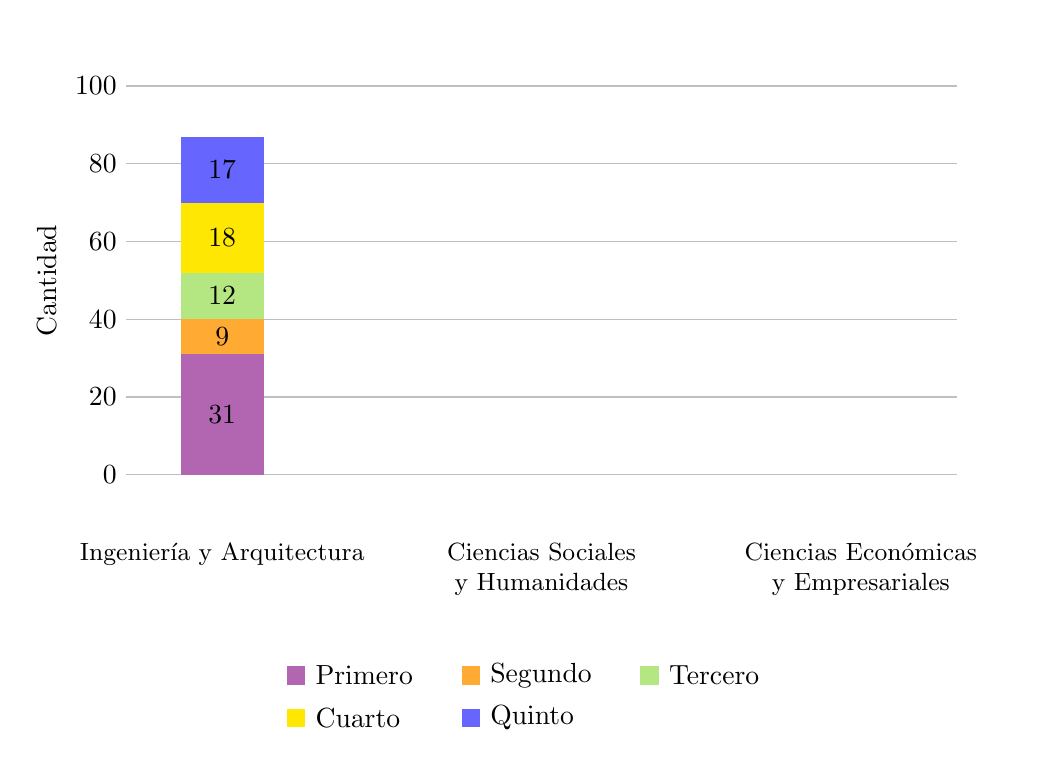
\begin{tikzpicture}
                \begin{axis}[
                    ybar stacked,
                    bar width=30pt,
                    nodes near coords,
                    enlargelimits=0.15,
                    ylabel={Cantidad},
                    symbolic x coords={Ingeniería y Arquitectura, Ciencias Sociales y Humanidades, Ciencias Económicas y Empresariales},
                    xtick=data,
                    x tick label style={rotate=0, anchor=north, align=center, text width=4cm, font=\small},
                    ymin=0,
                    ymax=100,
                    width=\textwidth,
                    height=8cm,
                    axis line style={draw=none},
                    tick style={draw=none},
                    ymajorgrids=true
                ]
                \addplot[fill=violet!60, draw=none] coordinates {(Ingeniería y Arquitectura,31) (Ciencias Sociales y Humanidades,0) (Ciencias Económicas y Empresariales,0)};
                \addplot[fill=myorange, draw=none] coordinates {(Ingeniería y Arquitectura,9) (Ciencias Sociales y Humanidades,0) (Ciencias Económicas y Empresariales,0)};
                \addplot[fill=mygreen, draw=none] coordinates {(Ingeniería y Arquitectura,12) (Ciencias Sociales y Humanidades,0) (Ciencias Económicas y Empresariales,0)};
                \addplot[fill=yellow!90!orange, draw=none] coordinates {(Ingeniería y Arquitectura,18) (Ciencias Sociales y Humanidades,0) (Ciencias Económicas y Empresariales,0)};
                \addplot[fill=blue!60, draw=none] coordinates {(Ingeniería y Arquitectura,17) (Ciencias Sociales y Humanidades,0) (Ciencias Económicas y Empresariales,0)};
                \end{axis}
                \matrix [draw=none, below, xshift=0cm, yshift=-0.5cm, anchor=north, ampersand replacement=\&, column sep=0.5cm] at (current bounding box.south) {
                    \node [fill=violet!60, label=right:Primero] {}; \& \node [fill=myorange, label=right:Segundo] {}; \& \node [fill=mygreen, label=right:Tercero] {}; \\
                    \node [fill=yellow!90!orange, label=right:Cuarto] {}; \& \node [fill=blue!60, label=right:Quinto] {}; \& \\
                };
            \end{tikzpicture}
            \caption{Grafico eAño de carrera y Facultad }
            \label{fig:anio_facultad}
        \end{figure}

        Como resultado de la encuesta realizada a 87 estudiantes, la mayor parte de los que respondieron la encuesta fueron estudiantes de primer año (35.63\%), todos pertenecientes a la Facultad de Ingeniería y Arquitectura (100\%). UCAChat estará especialmente orientado a apoyar a estudiantes de nuevo ingreso, quienes enfrentan mayor incertidumbre respecto a procesos institucionales clave como retiro de materias, diferidos, inscripción y ubicación de información académica, etc. Dado que estos estudiantes son quienes más necesitan orientación en su transición universitaria, la muestra resultante es coherente y adecuada para los fines de la investigación, garantizando que las conclusiones reflejen las necesidades de los estudiantes que más se beneficiaran con la implementación de UCAchat.

        \section{Uso de chatbot o inteligencia artificial y con qué frecuencia la utilizan }
        En esta parte se encuesto a varios estudiantes para conocer si han utilizado una inteligencia artificial o chatbot y tambien que tanto la utilizan. Los resultados fueron los siguientes:
        \begin{figure}[H]
            \centering
            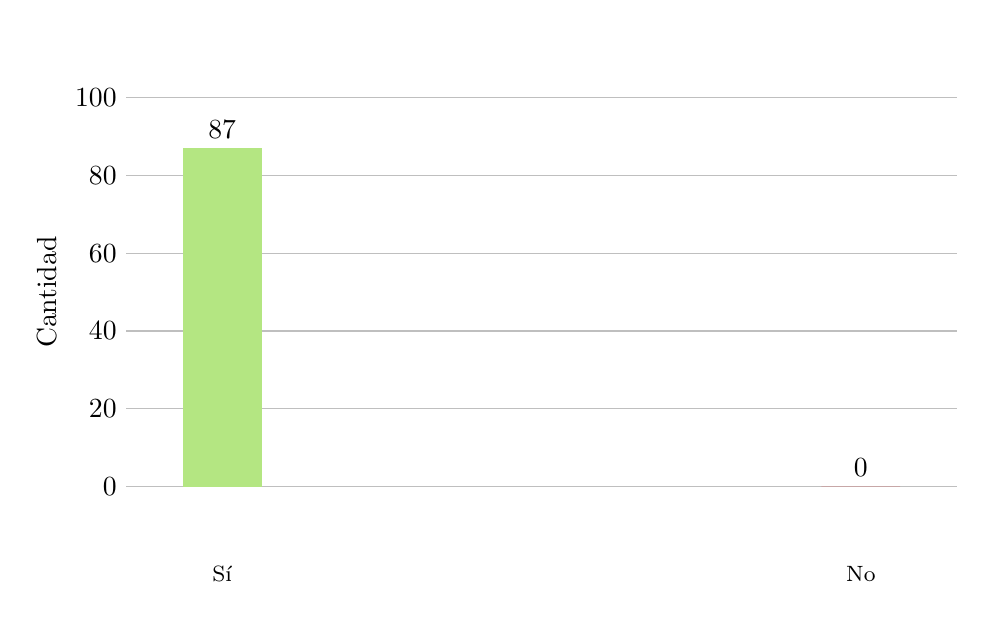
\begin{tikzpicture}
                \begin{axis}[
                    ybar,
                    bar width=1cm,
                    nodes near coords,
                    enlargelimits=0.15,
                    ylabel={Cantidad},
                    symbolic x coords={Si, No},
                    xtick={Si, No},
                    xticklabels={{S\'{i}}, {No}},
                    x tick label style={text width=2.5cm, align=center, font=\footnotesize},
                    ymin=0,
                    ymax=100,
                    width=\textwidth,
                    height=8cm,
                    bar shift=0pt,
                    axis line style={draw=none},
                    tick style={draw=none},
                    ymajorgrids=true
                ]
                \addplot[fill=mygreen, draw=none] coordinates {(Si,87)};
                \addplot[fill=red, draw=none] coordinates {(No,0)};
                \end{axis}
            \end{tikzpicture}
            \caption{Uso de la IA}
            \label{fig:uso_ia}
        \end{figure}
        
Los resultados muestran que todos los encuestados han utilizado IA y que su uso es frecuente, principalmente para actividades académicas como obtener información, realizar investigaciones y apoyar tareas. Esto evidencia una alta madurez tecnológica en la población estudiantil. Aunque la confianza en la IA es moderada lo cual es razonable, ya que siempre es necesario verificar la información no existe un rechazo hacia su uso. En conjunto, estos patrones confirman el potencial de UCAChat como asistente institucional, ya que los estudiantes están dispuestos a utilizar herramientas automatizadas siempre que ofrezcan información clara, precisa y verificable.

        \begin{figure}[H]
            \centering
            \resizebox{\textwidth}{!}{
            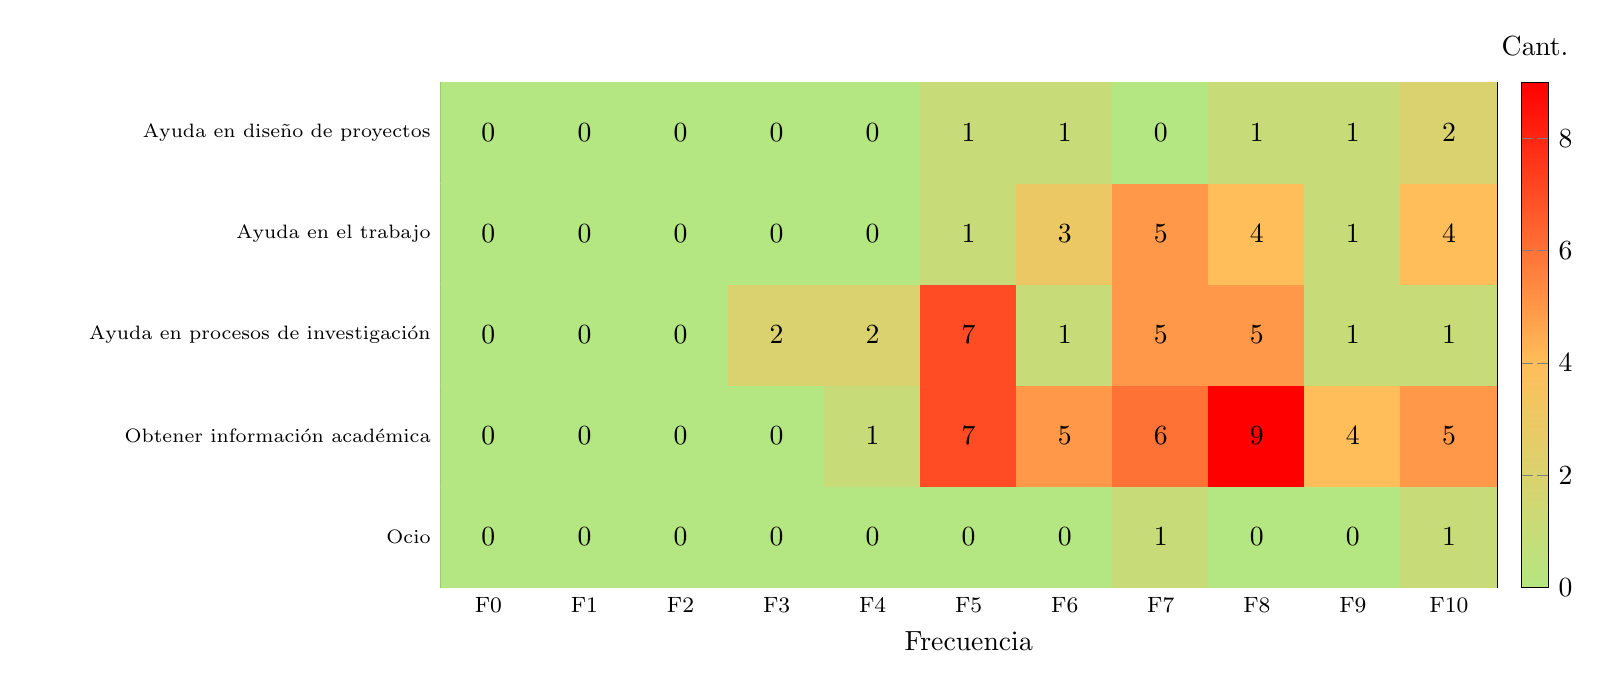
\begin{tikzpicture}
                \begin{axis}[
                    view={0}{90},
                    xlabel={Frecuencia},
                    xtick={0,1,2,3,4,5,6,7,8,9,10},
                    xticklabels={F0,F1,F2,F3,F4,F5,F6,F7,F8,F9,F10},
                    ytick={0,1,2,3,4},
                    yticklabels={Ocio, Obtener información académica, Ayuda en procesos de investigación, Ayuda en el trabajo, Ayuda en diseño de proyectos},
                    yticklabel style={text width=5cm, align=right, font=\scriptsize},
                    xticklabel style={font=\footnotesize},
                    colormap={semaforo}{color(0)=(mygreen); color(4)=(mylightorange); color(9)=(red)},
                    mesh/cols=11,
                    enlargelimits=false,
                    colorbar,
                    colorbar style={
                        title={Cant.},
                        width=10pt
                    },
                    point meta=explicit,
                    nodes near coords,
                    nodes near coords align={center},
                    width=15cm,
                    height=8cm
                ]
                \addplot [matrix plot*, mesh/rows=5] coordinates {
                    (0,0)[0] (1,0)[0] (2,0)[0] (3,0)[0] (4,0)[0] (5,0)[0] (6,0)[0] (7,0)[1] (8,0)[0] (9,0)[0] (10,0)[1]
                    (0,1)[0] (1,1)[0] (2,1)[0] (3,1)[0] (4,1)[1] (5,1)[7] (6,1)[5] (7,1)[6] (8,1)[9] (9,1)[4] (10,1)[5]
                    (0,2)[0] (1,2)[0] (2,2)[0] (3,2)[2] (4,2)[2] (5,2)[7] (6,2)[1] (7,2)[5] (8,2)[5] (9,2)[1] (10,2)[1]
                    (0,3)[0] (1,3)[0] (2,3)[0] (3,3)[0] (4,3)[0] (5,3)[1] (6,3)[3] (7,3)[5] (8,3)[4] (9,3)[1] (10,3)[4]
                    (0,4)[0] (1,4)[0] (2,4)[0] (3,4)[0] (4,4)[0] (5,4)[1] (6,4)[1] (7,4)[0] (8,4)[1] (9,4)[1] (10,4)[2]
                };
                \end{axis}
            \end{tikzpicture}
            }
            \caption{Mapa de calor Frecuencia x Uso}
            \label{fig:mapa_calor_frecuencia_uso}
        \end{figure} 

Los resultados muestran que la IA se utiliza principalmente con fines académicos y laborales. Las mayores frecuencias de uso aparecen en actividades relacionadas con trabajo e investigación, mientras que obtener información académica o diseño de proyectos también son comunes, aunque con una intensidad más moderada.

\section{Confianza en la respuesta de la Inteligencia Artificial}

En esta se les preguntó a los estudiantes en que tanto confían en la respuesta que les otorga la inteligencia artificial y también en que ámbito la utilizan, estos fueron los resultados: 

\begin{figure}[H]
    \centering
    \resizebox{\textwidth}{!}{
    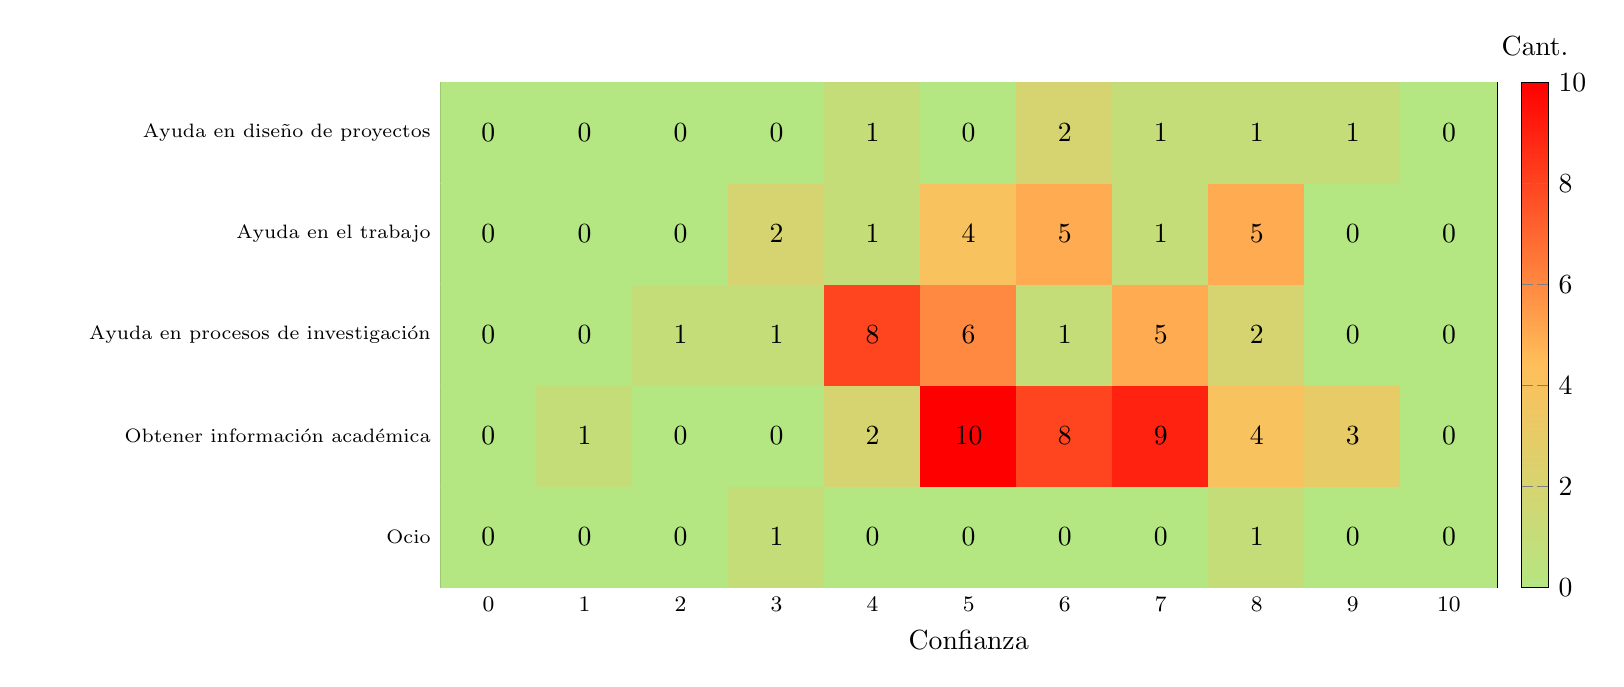
\begin{tikzpicture}
        \begin{axis}[
            view={0}{90},
            xlabel={Confianza},
            xtick={0,1,2,3,4,5,6,7,8,9,10},
            xticklabels={0,1,2,3,4,5,6,7,8,9,10},
            ytick={0,1,2,3,4},
            yticklabels={Ocio, Obtener información académica, Ayuda en procesos de investigación, Ayuda en el trabajo, Ayuda en diseño de proyectos},
            yticklabel style={text width=5cm, align=right, font=\scriptsize},
            xticklabel style={font=\footnotesize},
            colormap={semaforo}{color(0)=(mygreen); color(4)=(mylightorange); color(9)=(red)},
            mesh/cols=11,
            enlargelimits=false,
            colorbar,
            colorbar style={
                title={Cant.},
                width=10pt
            },
            point meta=explicit,
            nodes near coords,
            nodes near coords align={center},
            width=15cm,
            height=8cm
        ]
        \addplot [matrix plot*, mesh/rows=5] coordinates {
            (0,0)[0] (1,0)[0] (2,0)[0] (3,0)[1] (4,0)[0] (5,0)[0] (6,0)[0] (7,0)[0] (8,0)[1] (9,0)[0] (10,0)[0]
            (0,1)[0] (1,1)[1] (2,1)[0] (3,1)[0] (4,1)[2] (5,1)[10] (6,1)[8] (7,1)[9] (8,1)[4] (9,1)[3] (10,1)[0]
            (0,2)[0] (1,2)[0] (2,2)[1] (3,2)[1] (4,2)[8] (5,2)[6] (6,2)[1] (7,2)[5] (8,2)[2] (9,2)[0] (10,2)[0]
            (0,3)[0] (1,3)[0] (2,3)[0] (3,3)[2] (4,3)[1] (5,3)[4] (6,3)[5] (7,3)[1] (8,3)[5] (9,3)[0] (10,3)[0]
            (0,4)[0] (1,4)[0] (2,4)[0] (3,4)[0] (4,4)[1] (5,4)[0] (6,4)[2] (7,4)[1] (8,4)[1] (9,4)[1] (10,4)[0]
        };
        \end{axis}
    \end{tikzpicture}
    }
    \caption{Mapa de calor Confianza x Uso}
    \label{fig:mapa_calor_confianza_uso}
\end{figure}

Los resultados muestran que la confianza se sitúa en niveles medio-altos sin llegar a ser absoluta, lo que refleja un uso responsable en el que los estudiantes verifican la información obtenida.

\section{Tramites que les ha dificultado más a los estudiantes de la universidad}

Una de las preguntas que se realizo fue con respecto cuales son los tramites que para los estudiantes se les dificulta elaborar. Los resultados obtenidos fueron los siguientes: 

\begin{figure}[H]
    \centering
    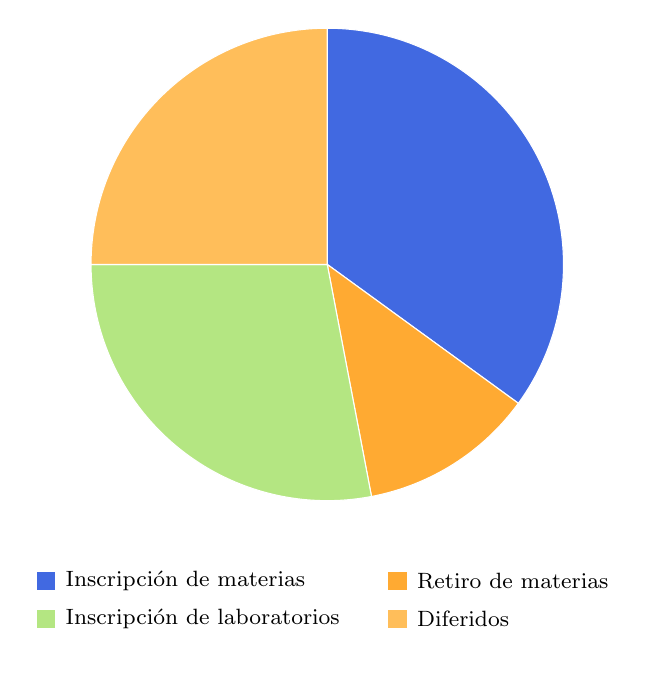
\begin{tikzpicture}
        \def\radius{3}
        % Inscripción de materias (MyBlue) - 35%
        \draw[fill=myblue, draw=white] (0,0) -- (90:\radius) arc (90:-36:\radius) -- cycle;
        
        % Retiro de materias (MyOrange) - 12%
        \draw[fill=myorange, draw=white] (0,0) -- (-36:\radius) arc (-36:-79.2:\radius) -- cycle;
        
        % Inscripción de laboratorios (MyGreen) - 28%
        \draw[fill=mygreen, draw=white] (0,0) -- (-79.2:\radius) arc (-79.2:-180:\radius) -- cycle;
        
        % Diferidos (mylightorange) - 25%
        \draw[fill=mylightorange, draw=white] (0,0) -- (-180:\radius) arc (-180:-270:\radius) -- cycle;
        
        % Legend
        \matrix [draw=none, below, xshift=0cm, yshift=-0.5cm, column sep=0.5cm, ampersand replacement=\&] at (current bounding box.south) {
            \node [fill=myblue, label=right:\footnotesize Inscripción de materias] {}; \&
            \node [fill=myorange, label=right:\footnotesize Retiro de materias] {}; \\
            \node [fill=mygreen, label=right:\footnotesize Inscripción de laboratorios] {}; \&
            \node [fill=mylightorange, label=right:\footnotesize Diferidos] {}; \\
        };
    \end{tikzpicture}
    \caption{Trámites con mayor dificultad}
    \label{fig:tramites_dificultad}
\end{figure}

En esta pregunta lo que se puede interpretar es la mayor dificultad a procesos asociados a la carga académica (inscripciones y laboratorios). Esto indica que los estudiantes encuentran obstáculos reiterados al momento de gestionar su matrícula. Los trámites relacionados con modificaciones posteriores (retiros, diferidos) también generan problemas, aunque en menor medida.

\section{Donde suelen los estudiantes buscar la información de la universidad}
La siguiente pregunta que se realizo fue en donde suelen los estudiantes buscar la información de la universidad y los resultados fueron los siguientes:

\begin{figure}[H]
    \centering
    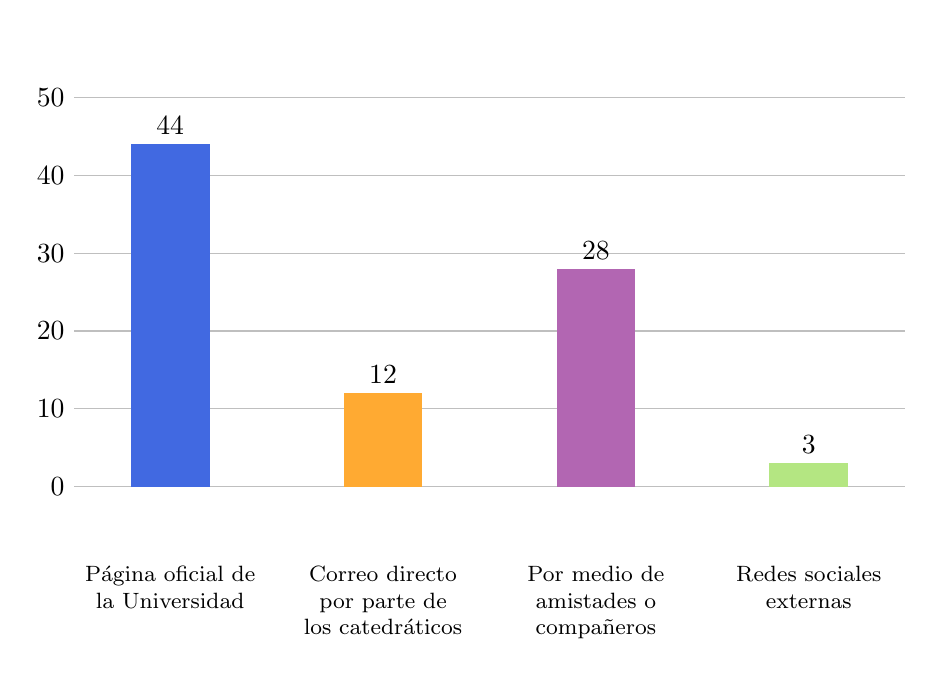
\begin{tikzpicture}
        \begin{axis}[
            ybar,
            bar width=1cm,
            width=\textwidth,
            height=8cm,
            symbolic x coords={Oficial, Correo, Amistades, Redes},
            xtick={Oficial, Correo, Amistades, Redes},
            xticklabels={{P\'{a}gina oficial de la Universidad}, {Correo directo por parte de los catedr\'{a}ticos}, {Por medio de amistades o compa\~{n}eros}, {Redes sociales externas}},
            x tick label style={text width=2.5cm, align=center, font=\footnotesize},
            nodes near coords,
            ymin=0,
            ymax=50,
            enlargelimits=0.15,
            ymajorgrids=true,
            axis line style={draw=none},
            tick style={draw=none},
            ytick={0,10,20,30,40,50},
            bar shift=0pt,
        ]
            \addplot[fill=myblue, draw=none] coordinates {(Oficial,44)};
            \addplot[fill=myorange, draw=none] coordinates {(Correo,12)};
            \addplot[fill=violet!60, draw=none] coordinates {(Amistades,28)};
            \addplot[fill=mygreen, draw=none] coordinates {(Redes,3)};
        \end{axis}
    \end{tikzpicture}
    \caption{Donde suelen los estudiantes buscar la información de la universidad}
    \label{fig:donde_buscan_info}
\end{figure}

Aunque el canal principal sigue siendo la página oficial, una parte notable de estudiantes depende de fuentes informales como compañeros. Esto sugiere que la información oficial podría resultar insuficiente o difícil de encontrar, por lo que los estudiantes recurren a alternativas más rápidas.

La universidad sí cuenta con un canal oficial, pero existe una brecha informativa que empuja a los estudiantes a consultar a sus pares, lo que puede generar inconsistencias o desinformación.

\section{Situación en buscar la información de la universidad}
        En esta sección se presentan los resultados obtenidos al consultar a los estudiantes sobre la facilidad o dificultad al buscar información de la universidad, utilizando una escala numérica.

        \begin{table}[H]
            \centering
            \caption{Situación en buscar la información de la universidad}
            \begin{tabular}{|l|c|c|}
                \hline
                \textbf{Tipo} & \textbf{Categoría} & \textbf{Frecuencia} \\ \hline
                Escala & 0 & 0 \\ \cline{2-3} 
                Numérica & 1 & 0 \\ \cline{2-3} 
                (0-10) & 2 & 7 \\ \cline{2-3} 
                 & 3 & 5 \\ \cline{2-3} 
                 & 4 & 6 \\ \cline{2-3} 
                 & 5 & 16 \\ \cline{2-3} 
                 & 6 & 20 \\ \cline{2-3} 
                 & 7 & 14 \\ \cline{2-3} 
                 & 8 & 10 \\ \cline{2-3} 
                 & 9 & 4 \\ \cline{2-3} 
                 & 10 & 5 \\ \hline
                \textbf{Total} & \multicolumn{1}{c|}{} & \textbf{87} \\ \hline
            \end{tabular}
            \label{tab:situacion_buscar_info}
        \end{table}

        Estos resultados reflejan una necesidad de mejora en la accesibilidad y claridad de la información institucional, lo que respalda la pertinencia de implementar un chatbot universitario como una herramienta que simplifique la búsqueda de información, reduzca el esfuerzo requerido por los estudiantes y mejore su experiencia general.

\section{Documentos que más se consultarían en UCAChat}
La siguiente pregunta es con relación a cuáles documentos los estudiantes consultarian en el chatbot UCAchat, los resultados fueron los siguientes:


\begin{figure}[H]
    \centering
    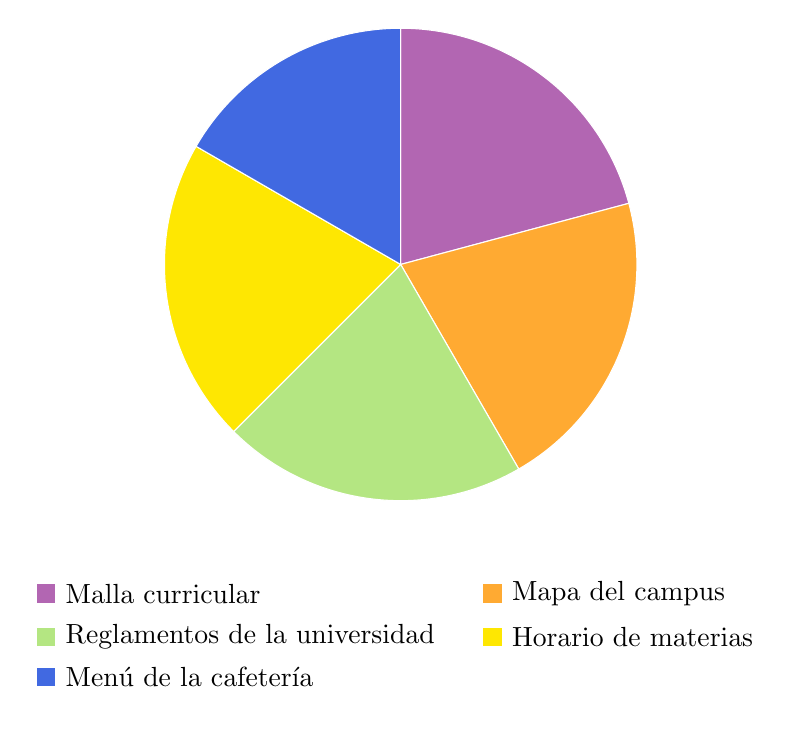
\begin{tikzpicture}
        \def\radius{3}
        % Purple - Malla curricular
        % Start 90, End 15
        \draw[fill=violet!60, draw=white] (0,0) -- (90:\radius) arc (90:15:\radius) -- cycle;
        
        % Orange - Mapa del campus
        % Start 15, End -60
        \draw[fill=myorange, draw=white] (0,0) -- (15:\radius) arc (15:-60:\radius) -- cycle;
        
        % Green - Reglamentos
        % Start -60, End -135
        \draw[fill=mygreen, draw=white] (0,0) -- (-60:\radius) arc (-60:-135:\radius) -- cycle;
        
        % Yellow - Horario
        % Start -135, End -210
        \draw[fill=yellow!90!orange, draw=white] (0,0) -- (-135:\radius) arc (-135:-210:\radius) -- cycle;
        
        % Blue - Menu
        % Start -210, End -270 (90)
        \draw[fill=myblue, draw=white] (0,0) -- (-210:\radius) arc (-210:-270:\radius) -- cycle;

        % Legend 2-2-1
        \matrix [draw=none, below, xshift=0cm, yshift=-0.5cm, anchor=north, ampersand replacement=\&, column sep=0.5cm] at (current bounding box.south) {
            \node [fill=violet!60, label=right:Malla curricular] {}; \& \node [fill=myorange, label=right:Mapa del campus] {}; \\
            \node [fill=mygreen, label=right:Reglamentos de la universidad] {}; \& \node [fill=yellow!90!orange, label=right:Horario de materias] {}; \\
            \node [fill=myblue, label=right:Men\'{u} de la cafeter\'{i}a] {}; \& \\
        };
    \end{tikzpicture}
    \caption{Documentos que más se consultarían en UCA Chat}
    \label{fig:docs_ucachat}
\end{figure}

Los resultados revelan que el interés principal de los estudiantes es acceder rápidamente a información académica y administrativa, especialmente aquella que influye directamente en:

La planificación de clases, la inscripción y carga académica, el cumplimiento de normas universitarias. 

Los documentos más solicitados corresponden a consultas frecuentes, lo que respalda la necesidad de un chatbot que centralice información dispersa o difícil de encontrar actualmente.


\section{Frecuencia estimada de uso de UCAChat}

En esta sección se presentan los resultados obtenidos al consultar a los estudiantes sobre la frecuencia estimada de uso del chatbot universitario UCAchat, utilizando una escala numérica.

\begin{table}[H]
    \centering
    \caption{Frecuencia de uso del chatbot universitario}
    \begin{tabular}{|l|c|c|}
        \hline
        \textbf{Tipo} & \textbf{Categoría} & \textbf{Frecuencia} \\ \hline
        Escala & 0 & 0 \\ \cline{2-3} 
        Numérica & 1 & 2 \\ \cline{2-3} 
        (0-10) & 2 & 6 \\ \cline{2-3} 
         & 3 & 5 \\ \cline{2-3} 
         & 4 & 8 \\ \cline{2-3} 
         & 5 & 13 \\ \cline{2-3} 
         & 6 & 14 \\ \cline{2-3} 
         & 7 & 10 \\ \cline{2-3} 
         & 8 & 15 \\ \cline{2-3} 
         & 9 & 9 \\ \cline{2-3} 
         & 10 & 5 \\ \hline
        \textbf{Total} & \multicolumn{1}{c|}{} & \textbf{87} \\ \hline
    \end{tabular}
    \label{tab:uso_ucachat}
\end{table}

Los resultados indican que UCAChat tendría una alta aceptación y un uso frecuente por parte de los estudiantes. Esta predisposición positiva refuerza la viabilidad de la implementación de UCAChat, ya que los estudiantes no solo están abiertos a utilizarlo, sino que lo perciben como una herramienta con potencial real para apoyar sus actividades académicas y administrativas, siempre que ofrezca información confiable y de fácil acceso.

\section{Características de confianza para el chatbot universitar}
Para garantizar la confianza en el uso de UCAChat, se consultó a los estudiantes sobre las características que consideran indispensables. Los resultados se detallan a continuación:

\begin{figure}[H]
    \centering
    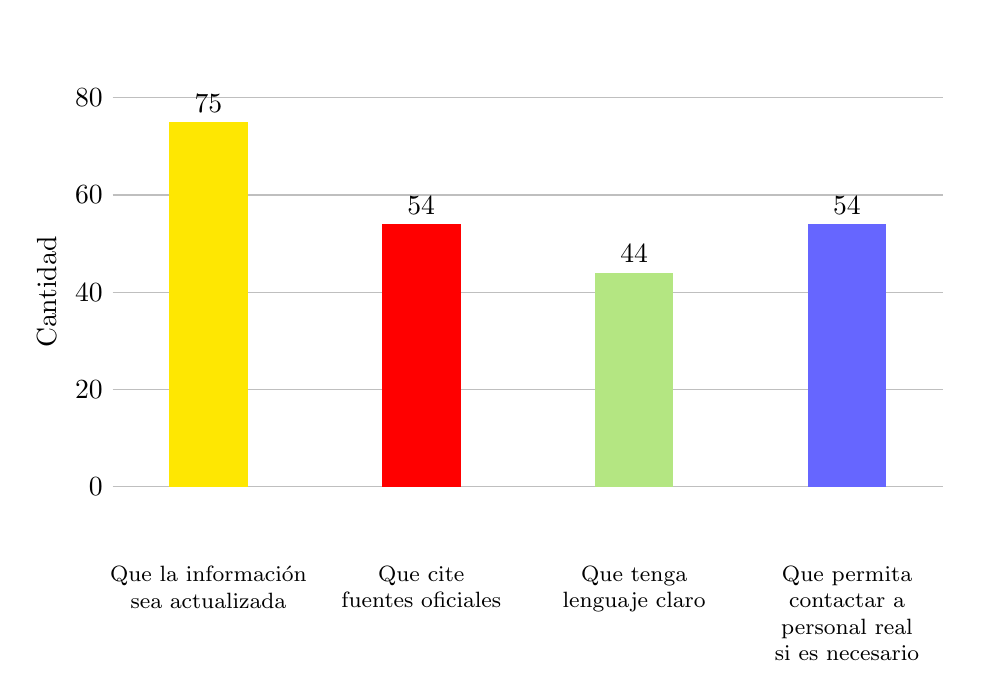
\begin{tikzpicture}
        \begin{axis}[
            ybar,
            bar width=1cm,
            nodes near coords,
            enlargelimits=0.15,
            ylabel={Cantidad},
            symbolic x coords={Actualizada, Fuentes, Claro, Contacto},
            xtick={Actualizada, Fuentes, Claro, Contacto},
            xticklabels={{Que la información sea actualizada}, {Que cite fuentes oficiales}, {Que tenga lenguaje claro}, {Que permita contactar a personal real si es necesario}},
            x tick label style={text width=2.5cm, align=center, font=\footnotesize},
            ymin=0,
            ymax=80,
            width=\textwidth,
            height=8cm,
            bar shift=0pt,
            axis line style={draw=none},
            tick style={draw=none},
            ymajorgrids=true
        ]
        \addplot[fill=yellow!90!orange, draw=none] coordinates {(Actualizada,75)};
        \addplot[fill=red, draw=none] coordinates {(Fuentes,54)};
        \addplot[fill=mygreen, draw=none] coordinates {(Claro,44)};
        \addplot[fill=blue!60, draw=none] coordinates {(Contacto,54)};
        \end{axis}
    \end{tikzpicture}
    \caption{Características de confianza para el chatbot universitario}
    \label{fig:confianza_chatbot}
\end{figure}

Los resultados evidencian que la actualización constante de la información es el factor más determinante para generar confianza en el chatbot universitario, al ser seleccionada por la gran mayoría de los encuestados. Esto refleja una preocupación clara por la vigencia y exactitud de los datos, especialmente en un entorno universitario donde los procesos, fechas y normativas pueden cambiar con frecuencia.

\section{Información que los estudiantes prefieren que UCAChat les proporcione}
La siguiente pregunta fue que tanta información les gustaría a los estudiantes ver en el chatbot de la universidad, estos fueron los resultados:

\begin{figure}[H]
    \centering
    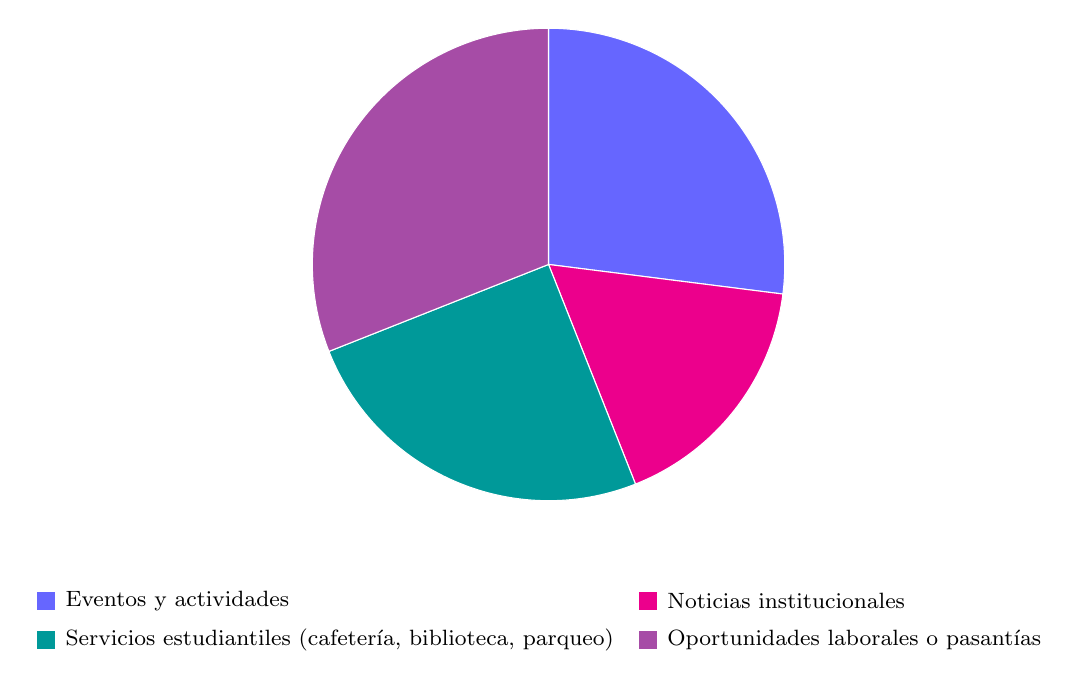
\begin{tikzpicture}
        \def\radius{3}
        % Blue - Eventos y actividades (~27%)
        % Start 90, End -7.2
        \draw[fill=blue!60, draw=white] (0,0) -- (90:\radius) arc (90:-7.2:\radius) -- cycle;
        
        % Pink - Noticias institucionales (~17%)
        % Start -7.2, End -68.4
        \draw[fill=magenta, draw=white] (0,0) -- (-7.2:\radius) arc (-7.2:-68.4:\radius) -- cycle;
        
        % Teal - Servicios estudiantiles (~25%)
        % Start -68.4, End -158.4
        \draw[fill=teal!80!cyan, draw=white] (0,0) -- (-68.4:\radius) arc (-68.4:-158.4:\radius) -- cycle;
        
        % Purple - Oportunidades (~31%)
        % Start -158.4, End -270 (90)
        \draw[fill=violet!70, draw=white] (0,0) -- (-158.4:\radius) arc (-158.4:-270:\radius) -- cycle;

        % Legend 2x2
        \def\servicesLabel{Servicios estudiantiles (cafeter\'{i}a, biblioteca, parqueo)}
        \matrix [draw=none, below, xshift=0cm, yshift=-0.5cm, anchor=north, ampersand replacement=\&, column sep=0.2cm] at (current bounding box.south) {
            \node [fill=blue!60, label=right:\footnotesize Eventos y actividades] {}; \& \node [fill=magenta, label=right:\footnotesize Noticias institucionales] {}; \\
            \node [fill=teal!80!cyan, label=right:{\footnotesize \servicesLabel}] {}; \& \node [fill=violet!70, label=right:{\footnotesize Oportunidades laborales o pasant\'{i}as}] {}; \\
        };
    \end{tikzpicture}
    \caption{Información proporcionada en el chatbot además de la académica}
    \label{fig:info_adicional_chatbot}
\end{figure}

Los resultados muestran Los resultados muestran que los estudiantes desean que el chatbot no solo brinde información académica, sino también contenido que les permita estar más conectados con la vida universitaria y resolver necesidades prácticas.

En conjunto, los resultados evidencian que los estudiantes buscan un chatbot integral, capaz de centralizar información académica, administrativa, de servicios y de vida universitaria, con un énfasis particular en herramientas que les ayuden a vincularse con oportunidades profesionales.

\section{Riesgos y preocupaciones que tendrá el estudiante al consultar el chatbot universitario}
En esta pregunta que se realizó a los estudiantes fue que tanto riesgos o preocupaciones tendrán al momento de hacer uso del chatbot universitario, los resultados se muestran en la Figura \ref{fig:riesgos_percibidos}.

\begin{figure}[H]
    \centering
    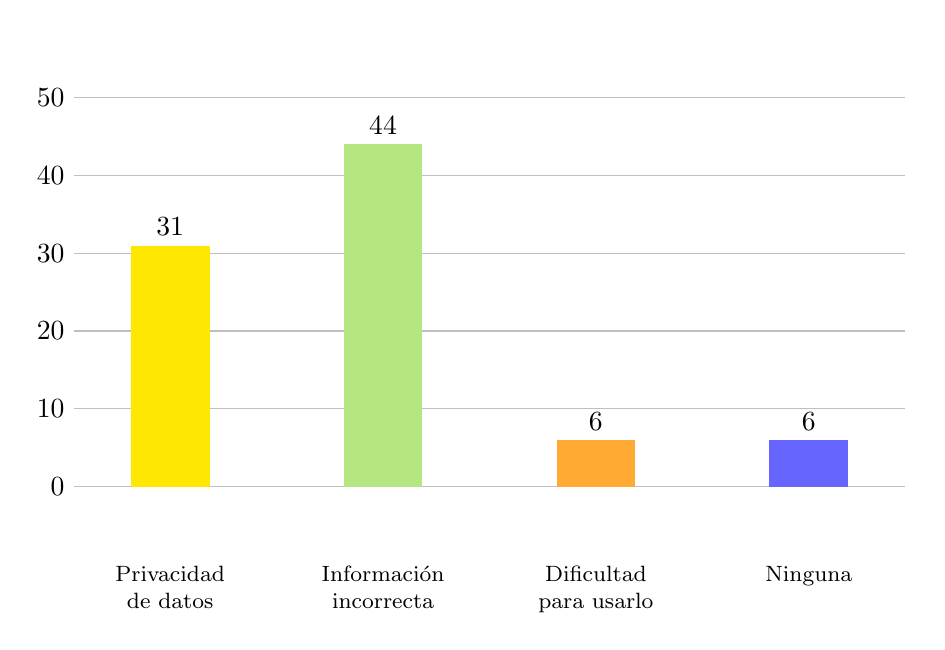
\begin{tikzpicture}
        \begin{axis}[
            ybar,
            bar width=1cm,
            width=\textwidth,
            height=8cm,
            symbolic x coords={Privacidad, Info, Dificultad, Ninguna},
            xtick={Privacidad, Info, Dificultad, Ninguna},
            xticklabels={{Privacidad de datos}, {Informaci\'{o}n incorrecta}, {Dificultad para usarlo}, {Ninguna}},
            x tick label style={text width=2.5cm, align=center, font=\footnotesize},
            nodes near coords,
            ymin=0,
            ymax=50,
            enlargelimits=0.15,
            ymajorgrids=true,
            axis line style={draw=none},
            tick style={draw=none},
            ytick={0,10,20,30,40,50},
            bar shift=0pt,
        ]
            % Privacidad - Yellow (~31)
            \addplot[fill=yellow!90!orange, draw=none] coordinates {(Privacidad,31)};
            
            % Info Incorrecta - Green (~44)
            \addplot[fill=mygreen, draw=none] coordinates {(Info,44)};
            
            % Dificultad - Orange (~6)
            \addplot[fill=myorange, draw=none] coordinates {(Dificultad,6)};
            
            % Ninguna - Blue (~6)
            \addplot[fill=blue!60, draw=none] coordinates {(Ninguna,6)};
        \end{axis}
    \end{tikzpicture}
    \caption{Riesgos percibidos}
    \label{fig:riesgos_percibidos}
\end{figure} 

\section{Satisfacción con los medios actuales para obtener la información de la universidad}
En esta sección se presentan los resultados obtenidos al consultar a los estudiantes sobre su nivel de satisfacción con los medios actuales para obtener información de la universidad, utilizando una escala numérica.

\begin{table}[H]
    \centering
    \caption{Satisfacción con los medios actuales para obtener la información de la universidad}
    \begin{tabular}{|l|c|c|}
        \hline
        \textbf{Tipo} & \textbf{Categoría} & \textbf{Frecuencia} \\ \hline
        Escala & 0 & 2 \\ \cline{2-3} 
        Numérica & 1 & 1 \\ \cline{2-3} 
        (0-10) & 2 & 6 \\ \cline{2-3} 
         & 3 & 1 \\ \cline{2-3} 
         & 4 & 9 \\ \cline{2-3} 
         & 5 & 16 \\ \cline{2-3} 
         & 6 & 17 \\ \cline{2-3} 
         & 7 & 16 \\ \cline{2-3} 
         & 8 & 12 \\ \cline{2-3} 
         & 9 & 5 \\ \cline{2-3} 
         & 10 & 2 \\ \hline
        \textbf{Total} & \multicolumn{1}{c|}{} & \textbf{87} \\ \hline
    \end{tabular}
    \label{tab:satisfaccion_medios_actuales}
\end{table}

Estos resultados reflejan una satisfacción moderada, lo que confirma la existencia de oportunidades de mejora en la forma en que la universidad comunica su información. Este escenario refuerza la pertinencia de implementar herramientas alternativas, como un chatbot universitario, que permitan mejorar la accesibilidad, claridad y rapidez en el acceso a la información institucional.

\section{Dificultad de los estudiantes en la comunicación con el personal administrativo o los catedráticos}
En esta sección se presentan los resultados obtenidos al consultar a los estudiantes sobre la dificultad que han experimentado al comunicarse con el personal administrativo o catedráticos, utilizando una escala numérica.

\begin{table}[H]
    \centering
    \caption{Dificultad de los estudiantes en la comunicación con el personal administrativo o los catedráticos}
    \begin{tabular}{|l|c|c|}
        \hline
        \textbf{Tipo} & \textbf{Categoría} & \textbf{Frecuencia} \\ \hline
        Escala & 0 & 3 \\ \cline{2-3} 
        Numérica & 1 & 5 \\ \cline{2-3} 
        (0-10) & 2 & 12 \\ \cline{2-3} 
         & 3 & 8 \\ \cline{2-3} 
         & 4 & 12 \\ \cline{2-3} 
         & 5 & 11 \\ \cline{2-3} 
         & 6 & 12 \\ \cline{2-3} 
         & 7 & 10 \\ \cline{2-3} 
         & 8 & 4 \\ \cline{2-3} 
         & 9 & 5 \\ \cline{2-3} 
         & 10 & 5 \\ \hline
        \textbf{Total} & \multicolumn{1}{c|}{} & \textbf{87} \\ \hline
    \end{tabular}
    \label{tab:dificultad_comunicacion}
\end{table}

Los resultados muestran que los estudiantes sí han experimentado dificultades para comunicarse con personal administrativo o catedráticos, aunque estas no se concentran exclusivamente en los niveles extremos. Las respuestas se distribuyen principalmente en valores medios de la escala (entre 4 y 6), lo que indica que la dificultad es moderada pero recurrente.

Destaca que una cantidad considerable de estudiantes ubicó su experiencia en los niveles 2, 4 y 6, lo cual refleja una percepción desigual: mientras algunos consideran que la comunicación es relativamente accesible, otros enfrentan obstáculos frecuentes. La presencia de respuestas en los valores altos (7 a 10) confirma que existe un grupo significativo que percibe la comunicación como complicada, especialmente cuando se requiere resolver dudas o trámites específicos.

\section{Preferencia del tipo de lenguaje para el chatbot}
La siguiente pregunta fue sobre qué tipo de lenguaje prefieren los estudiantes que use el chatbot, los resultados se muestran en la Figura \ref{fig:preferencia_lenguaje}.

\begin{figure}[H]
    \centering
    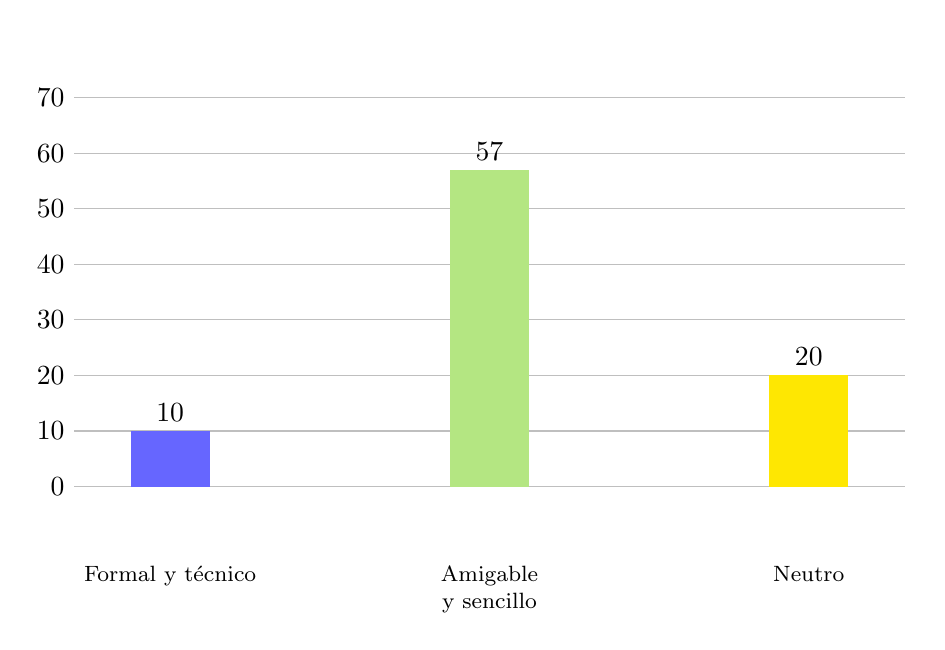
\begin{tikzpicture}
        \begin{axis}[
            ybar,
            bar width=1cm,
            width=\textwidth,
            height=8cm,
            symbolic x coords={Formal, Amigable, Neutro},
            xtick={Formal, Amigable, Neutro},
            xticklabels={{Formal y t\'{e}cnico}, {Amigable y sencillo}, {Neutro}},
            x tick label style={text width=2.5cm, align=center, font=\footnotesize},
            nodes near coords,
            ymin=0,
            ymax=70,
            enlargelimits=0.15,
            ymajorgrids=true,
            axis line style={draw=none},
            tick style={draw=none},
            ytick={0,10,20,30,40,50,60,70},
            bar shift=0pt,
        ]
            % Formal - Blue (10)
            \addplot[fill=blue!60, draw=none] coordinates {(Formal,10)};
            
            % Amigable - Green (57)
            \addplot[fill=mygreen, draw=none] coordinates {(Amigable,57)};
            
            % Neutro - Yellow (20)
            \addplot[fill=yellow!90!orange, draw=none] coordinates {(Neutro,20)};
        \end{axis}
    \end{tikzpicture}
    \caption{Preferencia en el lenguaje que use UCA Chat}
    \label{fig:preferencia_lenguaje}
\end{figure}

La mayoría de los estudiantes espera que el chatbot use un estilo amigable, cercano y claro, que facilite la comprensión y agilice las consultas. para que sea más comprensible para cualquier persona que ocupe el UCAChat.

\section{Preferencia de los estudiantes sobre la personalidad (nombre o avatar) que el chatbot maneje}
La siguiente pregunta fue sobre si los estudiantes prefieren que el chatbot tenga una personalidad definida (nombre o avatar), los resultados se muestran en la Figura \ref{fig:preferencia_personalidad}.

\begin{figure}[H]
    \centering
    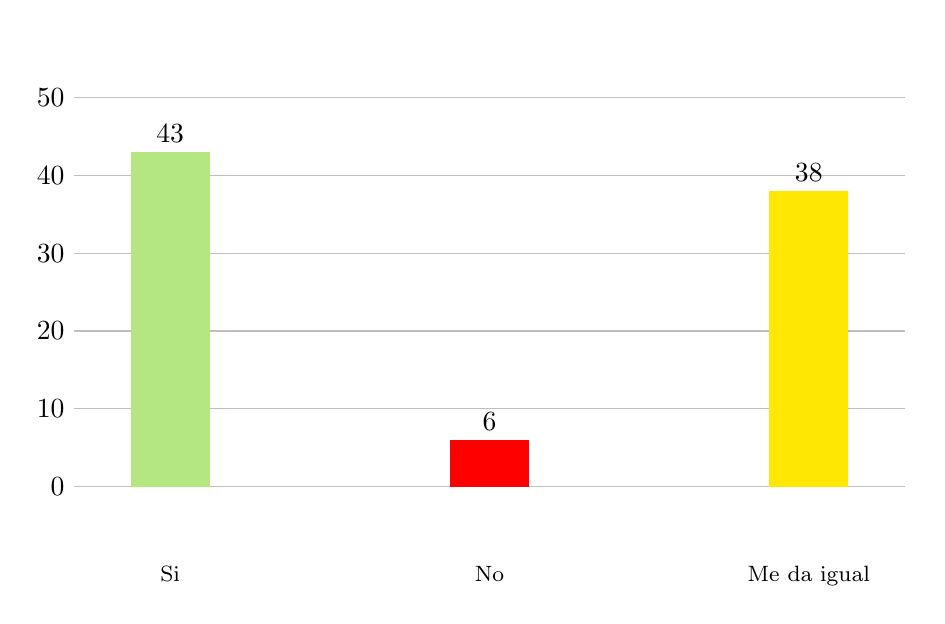
\begin{tikzpicture}
        \begin{axis}[
            ybar,
            bar width=1cm,
            width=\textwidth,
            height=8cm,
            symbolic x coords={Si, No, Igual},
            xtick={Si, No, Igual},
            xticklabels={Si, No, Me da igual},
            x tick label style={text width=2.5cm, align=center, font=\footnotesize},
            nodes near coords,
            ymin=0,
            ymax=50,
            enlargelimits=0.15,
            ymajorgrids=true,
            axis line style={draw=none},
            tick style={draw=none},
            ytick={0,10,20,30,40,50},
            bar shift=0pt,
        ]
            % Si - Green (43)
            \addplot[fill=mygreen, draw=none] coordinates {(Si,43)};
            
            % No - Red (6)
            \addplot[fill=red, draw=none] coordinates {(No,6)};
            
            % Igual - Yellow (38)
            \addplot[fill=yellow!90!orange, draw=none] coordinates {(Igual,38)};
        \end{axis}
    \end{tikzpicture}
    \caption{Preferencia en la personalidad de UcaChat}
    \label{fig:preferencia_personalidad}
\end{figure}

\section{Comodidad de los estudiantes al utilizar herramientas digitales o aplicaciones nuevas}
La siguiente pregunta fue para conocer qué tan cómodos se sienten los estudiantes al utilizar nuevas tecnologías, los resultados se muestran en la Figura \ref{fig:adaptacion_tecnologias}.

\begin{figure}[H]
    \centering
    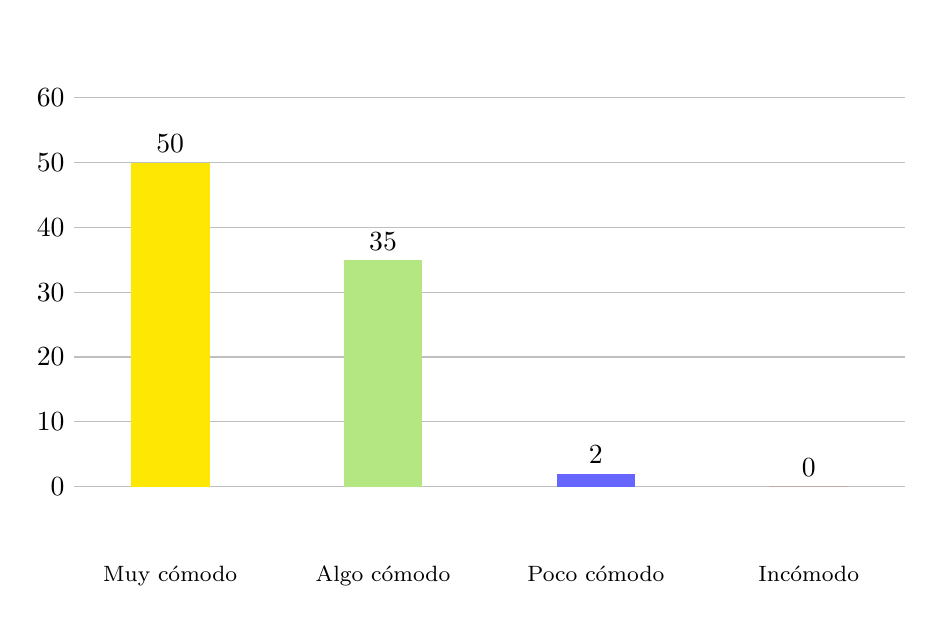
\begin{tikzpicture}
        \begin{axis}[
            ybar,
            bar width=1cm,
            width=\textwidth,
            height=8cm,
            symbolic x coords={Muy, Algo, Poco, Inc},
            xtick={Muy, Algo, Poco, Inc},
            xticklabels={{Muy c\'{o}modo}, {Algo c\'{o}modo}, {Poco c\'{o}modo}, {Inc\'{o}modo}},
            x tick label style={text width=2.5cm, align=center, font=\footnotesize},
            nodes near coords,
            ymin=0,
            ymax=60,
            enlargelimits=0.15,
            ymajorgrids=true,
            axis line style={draw=none},
            tick style={draw=none},
            ytick={0,10,20,30,40,50,60},
            bar shift=0pt,
        ]
            % Muy comodo - Yellow (50)
            \addplot[fill=yellow!90!orange, draw=none] coordinates {(Muy,50)};
            
            % Algo comodo - Green (35)
            \addplot[fill=mygreen, draw=none] coordinates {(Algo,35)};
            
            % Poco comodo - Blue (2)
            \addplot[fill=blue!60, draw=none] coordinates {(Poco,2)};

            % Incomodo - Red (0)
            \addplot[fill=red, draw=none] coordinates {(Inc,0)};
        \end{axis}
    \end{tikzpicture}
    \caption{Adaptación a nuevas tecnologías}
    \label{fig:adaptacion_tecnologias}
\end{figure}

Los resultados muestran que la población encuestada posee un alto nivel de familiaridad y adaptación tecnológica, lo cual facilita la adopción de nuevas plataformas institucionales, incluyendo un a UCAChat.

\section{Consideración sobre el uso de la Inteligencia Artificial en las universidades puede mejorar la experiencia estudiantil}
La siguiente pregunta fue para conocer la opinión de los estudiantes sobre si el uso de la IA en las universidades puede mejorar su experiencia, los resultados se muestran en la Figura \ref{fig:ia_mejora_experiencia}.

\begin{figure}[H]
    \centering
    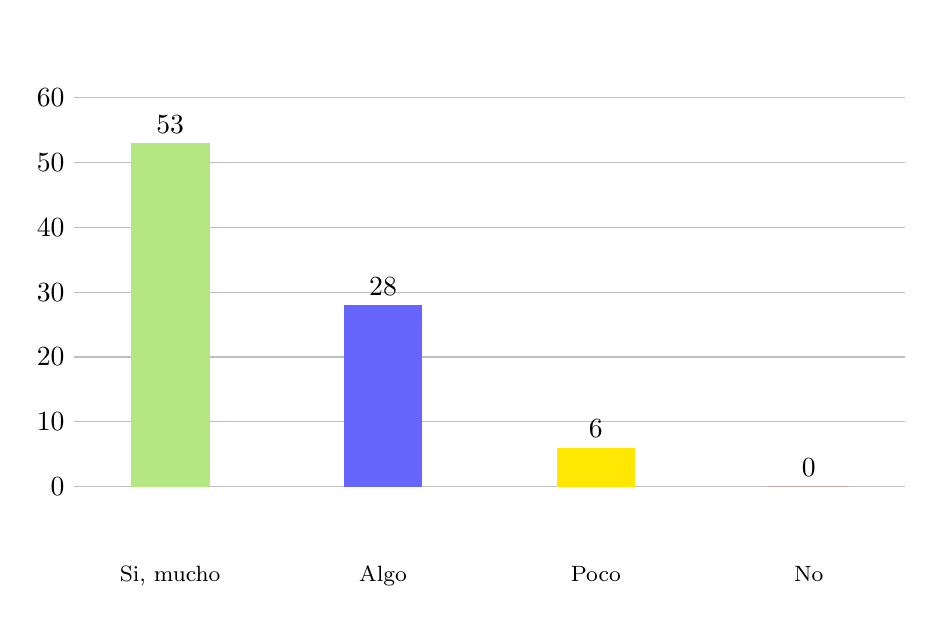
\begin{tikzpicture}
        \begin{axis}[
            ybar,
            bar width=1cm,
            width=\textwidth,
            height=8cm,
            symbolic x coords={Si, Algo, Poco, No},
            xtick={Si, Algo, Poco, No},
            xticklabels={{Si, mucho}, {Algo}, {Poco}, {No}},
            x tick label style={text width=2.5cm, align=center, font=\footnotesize},
            nodes near coords,
            ymin=0,
            ymax=60,
            enlargelimits=0.15,
            ymajorgrids=true,
            axis line style={draw=none},
            tick style={draw=none},
            ytick={0,10,20,30,40,50,60},
            bar shift=0pt,
        ]
            % Si, mucho - Green (53)
            \addplot[fill=mygreen, draw=none] coordinates {(Si,53)};
            
            % Algo - Blue (28)
            \addplot[fill=blue!60, draw=none] coordinates {(Algo,28)};
            
            % Poco - Yellow (6)
            \addplot[fill=yellow!90!orange, draw=none] coordinates {(Poco,6)};

            % No - Red (0)
            \addplot[fill=red, draw=none] coordinates {(No,0)};
        \end{axis}
    \end{tikzpicture}
    \caption{Consideración sobre si la IA puede mejorar la experiencia estudiantil}
    \label{fig:ia_mejora_experiencia}
\end{figure}

\section{Percepción sobre la reducción de tiempo en trámites}
En esta pregunta se consultó a los estudiantes si consideran que la implementación de UCAchat podría reducir el tiempo que invierten en realizar trámites, utilizando una escala numérica.

\begin{table}[H]
    \centering
    \caption{Frecuencia estimada de uso de UCAchat}
    \begin{tabular}{|l|c|c|}
        \hline
        \textbf{Tipo} & \textbf{Categoría} & \textbf{Frecuencia} \\ \hline
        Escala & 0 & 0 \\ \cline{2-3} 
        Numérica & 1 & 0 \\ \cline{2-3} 
        (0-10) & 2 & 1 \\ \cline{2-3} 
         & 3 & 3 \\ \cline{2-3} 
         & 4 & 3 \\ \cline{2-3} 
         & 5 & 12 \\ \cline{2-3} 
         & 6 & 9 \\ \cline{2-3} 
         & 7 & 12 \\ \cline{2-3} 
         & 8 & 16 \\ \cline{2-3} 
         & 9 & 14 \\ \cline{2-3} 
         & 10 & 17 \\ \hline
        \textbf{Total} & \multicolumn{1}{c|}{} & \textbf{87} \\ \hline
    \end{tabular}
    \label{tab:reduccion_tiempo_tramites}
\end{table}

La mayoría considera que un chatbot universitario tendría un impacto significativo en reducir los tiempos de trámites, reforzando su necesidad y utilidad dentro de la experiencia estudiantil. Esto valida la propuesta del proyecto.






        }
    \capitulo{Formato de los trabajos}{
    A continuación, se muestran las características principales del formato de trabajos de graduación creado por la facultad de ingeniería y arquitectura de la UCA.
    
    \begin{lista}
        \item \textbf{Partes del documento:}
        \begin{lista}
            \item Primera portada.
            \item Segunda portada.
            \item Agradecimientos (opcional).
            \item Dedicatorias (opcional).
            \item Resumen.
            \item Índice.
            \item Índice de figuras.
            \item Índice de tablas.
            \item Siglas.
            \item Abreviaturas.
            \item Nomenclatura.
            \item Capítulos.
            \item Glosario (opcional).
            \item Referencias.
            \item Anexos.
        \end{lista}

        \item \textbf{Formato general:}
        \begin{lista}
            \item Pagina tamaño carta.
            \item Margen de 2.5cm en todos lados.
            \item Borde de encuadernación de 1cm.
            \item Fuente Times New Roman 11pt.
            \item Interlineado 1.5pt.
            \item Espacio extra entre párrafos 0.
            \item Línea vacía entre párrafos.
            \item Todas las secciones deben comenzar en página impar.
            \item En todas las secciones que llevan título, el titulo se coloca al inicio de la página, en negrita, en mayúscula y centrado horizontalmente.
            \item Debe haber separación de una línea vacía entre el título y el texto.
        \end{lista}

        \item \textbf{Portadas:}
        \begin{lista}
            \item Texto centrado horizontalmente.
            \item Espacio igual entre los párrafos para que el texto ocupe todo el espacio disponible.
            \item Texto en mayúscula.
            \item Fuente tamaño 14pt.
            \item Logo de la primera portada 2.5cm de alto.
            \item En la primera portada los nombres de los integrantes van ordenados en orden alfabético basados en el primer apellido.
    \end{lista}

    \item \textbf{Agradecimientos:}
    \begin{lista}
        \item Extensión máxima una página.
    \end{lista}

    \item \textbf{Dedicatoria:}
    \begin{lista}
        \item Una por cada integrante.
        \item Extensión máxima una página.
        \item Debe llevar el nombre correspondiente del integrante al final de la página y alineado al lado derecho.
    \end{lista}

    \item \textbf{Resumen:}
    \begin{lista}
        \item Extensión de una a tres páginas.
    \end{lista}

    \item \textbf{Índice:}
    \begin{lista}
        \item El espacio horizontal entre el nombre de las secciones y el número de página debe estar lleno de puntos.
        \item Se permite hasta tres niveles de título.
        \item Los títulos de las secciones principales van en mayúscula.
        \item Al final se deben colocarlos anexos.
    \end{lista}

    \item \textbf{Índice de figuras e índice de tablas:}
    \begin{lista}
        \item Cada entrada del índice de figuras debe iniciar con la palabra “Figura” seguido del número de capitulo y el número correlativo de la figura.
        \item Cada entrada del índice de tablas debe iniciar con la palabra “Tabla” seguido del número de capitulo y el número correlativo de la tabla.
    \end{lista}

    \item\textbf{Siglas, abreviaturas y nomenclatura:}
    \begin{lista}
        \item Van separados en dos columnas, en la columna izquierda se coloca la sigla o palabra seguido de dos puntos y en la columna derecha se coloca la definición.
    \end{lista}

    \item\textbf{Figuras:}
    \begin{lista}
        \item Las figuras incluyen gráficos, diagramas, fotos, etc.
        \item El epígrafe va en la parte inferior centrado horizontalmente.
        \item Al inicio va la palabra “Figura” seguido del número de capitulo y número correlativo.
        \item En el epígrafe continuo a la descripción de la figura va la fuente.
        \item La fuente sigue el siguiente formato, “Fuente: [apellido autor, año]”.
        \item Si la figura es de elaboración propia se coloca, “Fuente: [Elaboración propia]”.
        \item Si la figura ha sido adaptada de alguna parte se coloca, “Adaptado de: [apellido autor, año]”.
        \item Las figuras se pueden colocar con orientación horizontal, en ese caso siempre de izquierda a derecha.
        \item Si la figura tiene orientación horizontal, el epígrafe se coloca en el lado derecho de la página.
    \end{lista}

    \item\textbf{Tabla:}
    \begin{lista}
        \item El epígrafe va en la parte superior, centrado horizontalmente.
        \item Al inicio va la palabra “Tabla” seguido del número de capitulo y número correlativo.
        \item La fuente se coloca en la parte inferior, centrada horizontalmente.
        \item La fuente sigue el siguiente formato, “Fuente: [apellido autor, año]”.
        \item Si la tabla es de elaboración propia se coloca, “Fuente: [Elaboración propia]”.
        \item Si la figura ha sido adaptada de alguna parte se coloca, “Adaptado de: [apellido autor, año]”.
        \item Las tablas se pueden colocar con orientación horizontal, en ese caso siempre de izquierda a derecha.
        \item Si la tabla tiene orientación horizontal, el epígrafe se coloca en el lado izquierdo de la página.
    \end{lista}

    \item\textbf{Ecuaciones:}
    \begin{lista}
        \item Las ecuaciones deben estar numeradas de la siguiente forma “(Ec.1.1)”.
    \end{lista}

    \item \textbf{Glosario:}
    \begin{lista}
        \item Tiene el mismo formato que las siglas, abreviaturas y nomenclatura.
    \end{lista}

    \item\textbf{Referencia:}
    \begin{lista}
        \item El formato de la referencia es en formato APA.
        \item No se coloca sangría en las líneas de cada una de las referencias.
        \item Las referencias van separadas horizontalmente por una línea vacía.
    \end{lista}

    \item\textbf{Portada anexos:}
    \begin{lista}
        \item Los anexos se enumeran utilizando letras.
        \item La portada de los anexos lleva dos partes, lleva la palabra “ANEXO” en mayúscula seguido de la letra correspondiente, el tamaño de fuente de esta parte es 20pt.
        \item El título del anexo en mayúscula, el tamaño de fuente de esta parte es 16pt.
        \item Todo el texto va centrado vertical y horizontalmente.
    \end{lista}

    \end{lista}
    }
}

%=================================================================
%       Sección editable para conclusiones y recomendaciones
% ================================================================
% ================= NO MODIFICAR LOS COMANDOS ===================
% ================================================================

\newenvironment{conclusiones}{
    \begin{listaenumerada}
        \item La implementación del prototipo UCAchat, basado en una arquitectura de Retrieval-Augmented Generation (RAG), demostró ser una solución viable y pertinente para centralizar la información académica y administrativa de la Universidad Centroamericana José Simeón Cañas. El uso de documentos institucionales como base de conocimiento permitió ofrecer respuestas más precisas, verificables y alineadas con la realidad universitaria, mitigando el riesgo de desinformación y alucinaciones propias de los modelos de lenguaje tradicionales.
        \item Los resultados obtenidos a partir de la encuesta aplicada a los estudiantes evidencian una alta aceptación y disposición al uso de herramientas basadas en inteligencia artificial, especialmente entre estudiantes de nuevo ingreso. Se identificó que los principales problemas actuales radican en la dispersión de la información y la dificultad para realizar trámites académicos, lo cual valida la necesidad de un asistente conversacional institucional que reduzca tiempos, facilite la toma de decisiones y mejore la experiencia estudiantil.
        \item El desarrollo del prototipo permitió comprobar que un chatbot universitario no solo puede funcionar como un canal informativo, sino también como un apoyo estratégico en la comunicación institucional, siempre que se acompañe de una adecuada gestión de la base de conocimiento y consideraciones éticas claras. En este sentido, UCAchat se posiciona como una herramienta complementaria al personal administrativo, capaz de fortalecer la autonomía del estudiante sin reemplazar la atención humana en procesos complejos.
    \end{listaenumerada}
}{}

\newenvironment{recomendaciones}{
    \begin{lista}
        \item Es esencial mantener al día el chatbot universitario conocido como UCAchat. Esto se debe a que en futuras versiones, el estudiante podría requerir la búsqueda de información reciente de la universidad o de un documento específico, lo cual podría no estar actualizado. Por lo tanto, será necesario mantener su actualización anualmente.
        \item Es necesario designar un equipo o un responsable institucional encargado de la administración de la base de conocimiento de UCAchat, con el fin de verificar la veracidad, coherencia y vigencia de la información divulgada. Esto permitirá la disminución del riesgo de desinformación y el incremento de la confianza de los estudiantes en las respuestas proporcionadas por el chatbot de la universidad.
    \end{lista}
}{}

%=================================================================
%                Sección editable para glosario
% ================================================================
% ================= NO MODIFICAR LOS COMANDOS ====================
% ================================================================

\newcommand{\mostrarglosario}{true}
\itemglosario{Big Data}{Concepto que hace referencia a conjuntos de datos tan grandes y complejos que precisan de aplicaciones informáticas no tradicionales de procesamiento de datos para tratarlos adecuadamente.}
\itemglosario{Blockchain}{Tecnología de registro distribuido que permite almacenar información de manera segura, transparente e inmutable mediante una cadena de bloques enlazados criptográficamente.}
\itemglosario{Chatbot}{Programa informático diseñado para simular una conversación con usuarios humanos, especialmente a través de Internet, utilizando texto o voz.}
\itemglosario{Embeddings}{Representaciones vectoriales de palabras o frases en un espacio numérico continuo, donde la cercanía entre vectores indica similitud semántica.}
\itemglosario{Fine-Tuning}{Proceso de ajuste fino en el que un modelo preentrenado se somete a un entrenamiento adicional con un conjunto de datos específico para especializarlo en una tarea determinada.}
\itemglosario{Focus Group}{Técnica de investigación cualitativa que reúne a un pequeño grupo de personas para discutir y analizar un tema, producto o servicio bajo la guía de un moderador.}
\itemglosario{Framework}{Entorno de trabajo o marco conceptual que ofrece un conjunto estandarizado de conceptos, prácticas y criterios para enfocar un tipo de problemática particular.}
\renewcommand{\glosariovacio}{false}
\newglossaryentry{glos:Alucinacion}{name={Alucinación}, type=glosario, description={Fenómeno en inteligencia artificial donde un modelo generativo produce información que parece plausible pero es incorrecta, ilógica o no está basada en los datos de entrada.}}
\newglossaryentry{glos:LLM}{name={LLM}, type=glosario, description={Modelo de inteligencia artificial generativa entrenado con vastas cantidades de datos textuales, capaz de entender, resumir, traducir y predecir nuevo contenido.}}
\newglossaryentry{glos:RAG}{name={RAG}, type=glosario, description={Técnica que optimiza la salida de un LLM al permitirle consultar una base de conocimientos externa confiable antes de generar una respuesta.}}
\itemglosario{Transformers}{Arquitectura de aprendizaje profundo que utiliza mecanismos de atención para procesar secuencias de datos, permitiendo modelar dependencias a largo plazo en el texto.}
\itemglosario{Token}{Unidad básica de texto (puede ser una palabra, una parte de una palabra o un carácter) que un modelo de lenguaje procesa individualmente.}

%=================================================================
%                    Sección editable para anexos
% ===============================================================
% ================== NO MODIFICAR LOS COMANDOS ==================
% ================================================================

\newcommand{\anexos}{
    \anexo{anexos}{
     En los anexos se colocan los documentos, gráficos, tablas, imágenes u otros materiales complementarios que proporcionan información adicional relevante, pero que no forman parte del cuerpo principal del trabajo.
    }
}



%============================ENTORNOS============================%

% Entorno que contendra las secciones que llevan numeracion romana
\newenvironment{romanos}{
    \clearpage
    \pagenumbering{roman}
}{
    \paroimpar{\value{page}}
}

% Entorno que contendra las secciones que llevan numeracion arabiga
\newenvironment{arabigos}{
    \clearpage
    \pagenumbering{arabic}
}{
    \paroimpar{\value{page}}
}

%Creacion de entorno "portadas" que funciona para las dos portadas
\newenvironment{portadas}{
    \thispagestyle{empty} % Oculta el numero de pagina
    \begin{center} % Centra horizontalmente el texto
    
    \fontsize{14}{21}\selectfont % estáblece tamaño de fuente 14 y un interlineado de 21pts
}{
    \end{center} % Termina el entorno de texto centrado
    \newpage % Se crea un salto de pagina
}

%Creacion de entorno "primera portada" que utiliza el entorno "portadas"
\newenvironment{primeraportada}{

    % Se utiliza el entono "portadas" previamente creado
    \begin{portadas}
        %NOMBRE DE LA UNIVERSIDAD
        UNIVERSIDAD CENTROAMERICANA\\
        JOSÉ SIMEÓN CAÑAS\\
        \vspace{1.5\baselineskip}
        
        %LOGO DE LA UCA
        \begin{figure}[H] % El argumento [H] fuerza la posición exacta
            \centering
            \includegraphics[height=2.5cm]{img/Logo_UCA_2015.jpg}
        \end{figure}
        \vspace{- 10pt}
        \vspace{0.5\baselineskip}
        
        %TÍTULO DE LA TESIS
        \verificarvacio{\titulo}{ERROR: No se ha ingresado el título}{ERROR: El comando título no está definido}

        \vspace*{\fill}
        
        %FACULTAD
        TRABAJO DE GRADUACIÓN PREPARADO PARA LA\\ FACULTAD DE INGENIERÍA Y ARQUITECTURA\\
        \vspace*{\fill}
        
        %GRADO
        \verificarsexoautores
        \ifdefined\carrera
            \ifthenelse{\equal{\carrera}{}}{
                \textcolor{red}{\MakeUppercase{ERROR: El numero correspondiente a la carrera no se ha ingresado}}
            }
                {PARA OPTAR AL GRADO DE\\ \determinarcarrera{\carrera}{2}}
        \else
            \textcolor{red}{\MakeUppercase{ERROR: El comando carrera no esta definido}}
        \fi
        
        \vspace*{\fill}
        
        %ESTUDIANTES
        POR:\\
        \ifthenelse{\equal{\autorA}{} \AND \equal{\autorB}{} \AND \equal{\autorC}{} \AND \equal{\autorD}{}}{\textcolor{red}{\MakeUppercase{ERROR: No se ha ingresado ningún integrante del grupo\\}} \vspace*{\fill}}{
        \ifthenelse{\equal{\autorA}{}}{}{\MakeUppercase{\autorA}\\}
        \ifthenelse{\equal{\autorB}{}}{}{\MakeUppercase{\autorB}\\}
        \ifthenelse{\equal{\autorC}{}}{}{\MakeUppercase{\autorC}\\}
        \ifthenelse{\equal{\autorD}{}}{}{\MakeUppercase{\autorD}\\}

        \vspace*{\fill}}
        
        %FECHA
        \verificarvacio{\mesdegraduacion}{ERROR: No se ha ingresado la fecha de graduacion}{ERROR: El comando fecha no está definido}\\
        
        % UBICACION DE LA UNIVERSIDAD
        ANTIGUO CUSCATLÁN, EL SALVADOR, C.A.
        \vspace{-8.25pt}
        }
{
    \end{portadas} %Se termina entorno de portadas
}

%Se crea nuevo entorno "segunda portada" que utiliza el entorno "portadas"
\newenvironment{segundaportada}{
    % Se utiliza el entono "portadas" previamente creado
    \begin{portadas}
    
        %SEXO DEL RECTOR O RECTORA
        \ifdefined\sexorector
            \ifthenelse{\equal{\sexorector}{}}{\textcolor{red}{
            \MakeUppercase{ERROR: No se ha ingresado el sexo del rector}}}{
                \ifthenelse{\equal{\sexorector}{masculino}}{
                    \MakeUppercase{rector}
                }{
                    \ifthenelse{\equal{\sexorector}{femenino}}{
                        \MakeUppercase{rectora}
                    }{
                        \textcolor{red}{
                            \MakeUppercase{ERROR: El sexo del rector solo puede ser "masculino" o "femenino"}
                        }
                    }
                }
            }\\
        \else
            \textcolor{red}{\MakeUppercase{ERROR: el comando sexorector no está definido}}
        \fi

        %NOMBRE DEL RECTOR
        \verificarvacio{\rector}{ERROR: No se ha ingresado el nombre del rector}{ERROR: El comando rector no está definido}\\
        \vspace*{\fill}
        
        %SEXO DEL SECRETARIO O SECRETARIA
        \ifdefined\sexosecretario
            \ifthenelse{\equal{\sexosecretario}{}}{\textcolor{red}{
            \MakeUppercase{ERROR: No se ha ingresado el sexo del secretario general}}}{
                \ifthenelse{\equal{\sexosecretario}{masculino}}{
                    \MakeUppercase{Secretario general}
                }{
                    \ifthenelse{\equal{\sexosecretario}{femenino}}{
                        \MakeUppercase{Secretaria general}
                    }{
                        \textcolor{red}{
                            \MakeUppercase{ERROR: El sexo del secretario solo puede ser "masculino" o "femenino"}
                        }
                    }
                }
            }\\
        \else
            \textcolor{red}{\MakeUppercase{ERROR: El comando sexosecretario no está definido}}
        \fi
        
        %NOMBRE DEL SECRETARIO O SECRETARIA
        \verificarvacio{\secretariogeneral}{ERROR: No se ha ingresado el nombre del secretario general}{ERROR: El comando secretariogeneral no está definido}\\
        \vspace*{\fill}
        
        %SEXO DEL DECANO O DECANA
        \ifdefined\sexodecano
            \ifthenelse{\equal{\sexodecano}{}}{\textcolor{red}{
            \MakeUppercase{ERROR: No se ha ingresado el sexo del decano}}}{
                \ifthenelse{\equal{\sexodecano}{masculino}}{
                    \MakeUppercase{decano de la facultad de ingeniería y arquitectura}
                }{
                    \ifthenelse{\equal{\sexodecano}{femenino}}{
                        \MakeUppercase{decana de la facultad de ingeniería y arquitectura}
                    }{
                        \textcolor{red}{
                            \MakeUppercase{ERROR: El sexo del decano solo puede ser "masculino" o "femenino"}
                        }
                    }
                }
            }\\
         \else
            \textcolor{red}{\MakeUppercase{ERROR: El comando sexodecano no está definido}}\\
        \fi

        %NOMBRE DEL DECANO
        \verificarvacio{\decano}{ERROR: No se ha ingresado el nombre del decano}{ERROR: El comando decano no está definido}\\
        \vspace*{\fill}

        %SEXO DEL DIRECTOR DE LA CARRERA
        \ifdefined\sexodirectordecarrera
            \ifthenelse{\equal{\sexodirectordecarrera}{}}{\textcolor{red}{
            \MakeUppercase{ERROR: No se ha ingresado el sexo del director de la carrera}}}{
                \ifthenelse{\equal{\sexodirectordecarrera}{masculino}}{
                    DIRECTOR DE LA CARRERA DE\determinarcarrera{\carrera}{1}
                }{
                    \ifthenelse{\equal{\sexodirectordecarrera}{femenino}}{
                        DIRECTORA DE LA CARRERA DE\determinarcarrera{\carrera}{\masMujeres}{1}
                    }{
                        \textcolor{red}{
                            \MakeUppercase{ERROR: El sexo del director de carrera solo puede ser "masculino" o "femenino"}
                        }
                    }
                }
            }
            \\
        \else
            \textcolor{red}{\MakeUppercase{ERROR: El comando sexodirectordecarrera no está definido}}\\
        \fi

        %NOMBRE DEL DIRECTOR DE CARRERA
        \verificarvacio{\directordecarrera}{ERROR: No se ha ingresado el nombre del director de carrera}{ERROR: El comando directordecarrera no está definido}\\
        \vspace*{\fill}
        
        %DIRECTOR DEL TRABAJO
        \ifdefined\sexodirectordetrabajo
            \ifthenelse{\equal{\sexodirectordetrabajo}{}}{\textcolor{red}{
            \MakeUppercase{ERROR: No se ha ingresado el sexo del director del trabajo}}}{
                \ifthenelse{\equal{\sexodirectordetrabajo}{masculino}}{
                    \MakeUppercase{Director del trabajo}
                }{
                    \ifthenelse{\equal{\sexodirectordetrabajo}{femenino}}{
                        \MakeUppercase{Directora del trabajo}
                    }{
                        \textcolor{red}{
                            \MakeUppercase{ERROR: El sexo del director del trabajo solo puede ser "masculino" o "femenino"}
                        }
                    }
                }
            }\\
        \else
            \textcolor{red}{\MakeUppercase{ERROR: El comando sexodirectordetrabajo no está definido}}\\
        \fi

        %NOMBRE DEL DIRECTOR DE TRABAJO DE GRADUACION
        \verificarvacio{\directordetrabajo}{ERROR: No se ha ingresado el nombre del director del trabajo}{ERROR: El comando directordetrabajo no está definido}\\
        \vspace*{\fill}
        
        %SEXO DEL LECTOR O LECTORA
        \ifdefined\sexolector
            \ifthenelse{\equal{\sexolector}{}}{\textcolor{red}{
            \MakeUppercase{ERROR: No se ha ingresado el sexo del lector}}}{
                \ifthenelse{\equal{\sexolector}{masculino}}{
                    \MakeUppercase{lector}
                }{
                    \ifthenelse{\equal{\sexolector}{femenino}}{
                        \MakeUppercase{lectora}
                    }{
                        \textcolor{red}{
                            \MakeUppercase{ERROR: El sexo del lector solo puede ser "masculino" o "femenino"}
                        }
                    }
                }
            }\\
        \else
            \textcolor{red}{\MakeUppercase{ERROR: El comando sexolector no está definido}}\\
        \fi
        
        %NOMBRE DEL LECTOR O LECTORA
        \verificarvacio{\lector}{ERROR:No se ha ingresado el nombre del lector}{ERROR: El comando lector no está definido}\\
        }
{
    \end{portadas} %Se termina entorno de portadas
}

% Se crea el entorno que se utilizara para el agradecimiento
\newenvironment{agradecimientoentorno}{
    %Se valida si el comando agradecimiento está definido
    \ifdefined\agradecimiento
        %Se valida si el comando agradecimiento está vacío
        \ifthenelse{\equal{\agradecimiento}{}}{}{
        \thispagestyle{empty} % Oculta el numero de pagina
        
        {\centering\textbf{AGRADECIMIENTOS}\par} % Título en negrita y mayúsculas
        
        \setcounter{agradecimientoinicio}{\value{page}}
        
        \agradecimiento % Muestra el agradecimiento si está presente
        
        \setcounter{agradecimientofinal}{\value{page}}
        
         \setcounter{agradecimientodiferencia}{\value{agradecimientofinal}}
         
        \addtocounter{agradecimientodiferencia}{-\value{agradecimientoinicio}}

         %Validar si el agradecimiento ocupa mas de una pagina
         \ifthenelse{\value{agradecimientodiferencia} < 1}{
            
        }{
            \textcolor{red}{\MakeUppercase{ERROR: El agradecimiento no puede ocupar más de una pagina}}
        }
        }
    \else
        \thispagestyle{empty}
        \textcolor{red}{\MakeUppercase{ERROR: El comando agradecimiento no está definido}}\\
    \fi
}{
    
}

% Se crea nuevo entorno para dedicatoria individuales
\newenvironment{dedicatoriasimple}[2]{
    \chapter*{\phantom{Dedicatoria \thepage}}
    \thispagestyle{empty}

    %Se guarda el numero de pagina inicial de cada dedicatoria en un contador
    \setcounter{dedicatoriasimpleinicio}{\value{page}}
        
    {\centering\textbf{DEDICATORIA}\par} % Título en negrita y mayúsculas

        #1 % Texto de la dedicatoria
        
    \begin{flushright} %Anilea el texto a la derecha
        #2\\ % Nombre del integrante del grupo que escribio la dedicatoria
    \end{flushright}

    %Se guarda el numero de pagina final de cada dedicatoria en un contador
    \setcounter{dedicatoriasimplefinal}{\value{page}}
}{
    % Verifica si la dedicatoria ocupa más de una pagina
    \setcounter{dedicatoriasimplediferencia}{\value{dedicatoriasimplefinal}}
    
    \addtocounter{dedicatoriasimplediferencia}{-\value{dedicatoriasimpleinicio}}
    \ifthenelse{\value{dedicatoriasimplediferencia} < 1}{
        %Si la dedicatoria ocupa solo una pagina entonces no hace nada
    }{
    % Sin la dedicatoria ocupa más de una pagina entonces se muestra 
    % advertencia en rojo
    \textcolor{red}{\MakeUppercase{ERROR: La dedicatoria no puede ocupar más de una pagina}}
    }
}

%Se crea entorno principal para mostrar las dedicatorias
\newenvironment{dedicatoria}{
     %Valida si el comando "dedicatoriaautorA" esta definida
    \ifdefined\dedicatoriaautorA
        %Valida si el comando "dedicatoriaautorA" es true
        \ifthenelse{\equal{\dedicatoriaautorA}{}}{

        }{
            \begin{dedicatoriasimple}
                {\dedicatoriaautorA}
                {\autorA}
            \end{dedicatoriasimple}
        }
        \else
            \thispagestyle{empty}
            \textcolor{red}{\MakeUppercase{ERROR: El comando dedicatoriaautorA no está definido}}
        \fi

        %Valida si el comando "dedicatoriaautorB" esta definida
        \ifdefined\dedicatoriaautorB
            %Valida si el comando "dedicatoriaautorB" es true
            \ifthenelse{\equal{\dedicatoriaautorB}{}}{

            }{
                \begin{dedicatoriasimple}
                {\dedicatoriaautorB}
                {\autorB}
                \end{dedicatoriasimple}
            }
        \else
            \thispagestyle{empty}
            \textcolor{red}{\MakeUppercase{ERROR: El comando dedicatoriaautorB no está definido}}
        \fi

        %Valida si el comando "dedicatoriaautorC" esta definida
        \ifdefined\dedicatoriaautorC
            %Valida si el comando "dedicatoriaautorC" es true
            \ifthenelse{\equal{\dedicatoriaautorC}{}}{
   
            }{
                \begin{dedicatoriasimple}
                {\dedicatoriaautorC}
                {\autorC}
                \end{dedicatoriasimple}
            }
        \else
            \thispagestyle{empty}
            \textcolor{red}{\MakeUppercase{ERROR: El comando dedicatoriaautorC no está definido}}
        \fi
        
        %Valida si el comando "dedicatoriaautorC" esta definida
        \ifdefined\dedicatoriaautorD
            %Valida si el comando "dedicatoriaautorC" es true
            \ifthenelse{\equal{\dedicatoriaautorD}{}}{
                
            }{
                \begin{dedicatoriasimple}
                {\dedicatoriaautorD}
                {\autorD}
                \end{dedicatoriasimple}
            }
        \else
            \thispagestyle{empty}
            \textcolor{red}{\MakeUppercase{ERROR: El comando dedicatoriaautorA no está definido}}
        \fi
        
    }
{

}

%Se crea un nuevo entorno para el resumen
\newenvironment{resumenentorno}{
    %Se valida si el comando "resumen" esta definido
    \ifdefined\resumen
        %Se valida si el comando "resumen" esta vacío
        \ifthenelse{\equal{\resumen}{}}{
            \textcolor{red}{\MakeUppercase{ERROR: No se ha ingresado el resumen.}} % Muestra un mensaje de error en rojo
        }{
            \setcounter{resumeninicio}{\value{page}} %Se agrega el numero de la pagina inicial en el contador
            
            {\centering\textbf{RESUMEN}\par}
            \resumen
    
            \setcounter{resumenfinal}{\value{page}} %Se agrega el numero de la pagina final en el contador         
        }
    \else
        \textcolor{red}{\MakeUppercase{ERROR: El comando resumen no está definido}}
    \fi
}{
    %Se establece el valor de la diferencia entre el contador final y el inicial y se guarda en el contador "resumendiferencia"
     \setcounter{resumendiferencia}{\value{resumenfinal}} 
     \addtocounter{resumendiferencia}{-\value{resumeninicio}}

    \ifthenelse{\value{resumendiferencia} < 0 \or \value{resumendiferencia} > 2}{
        %Si el resumen solo ocupa una pagina o más de tres paginas, entonces se muestra un error
        \textcolor{red}{\MakeUppercase{ERROR: La extensión del resumen debe ser de 2 a 3 paginas.}}
    }{
      
    }
}

%Se crea un entorno para el indice
\newenvironment{indice}{

    \renewcommand{\contentsname}{
        \vspace{-\baselineskip}
        {\centering \fontsize{11}{16.5}\selectfont ÍNDICE\\ \vspace{\baselineskip}}
        } %Se coloca el indice del título centrado y en mayuscula
        
    \vspace*{-\topskip}
    \vspace*{-\headsep}
    
    \tableofcontents %Se muestra el indice
    
}{

}

%Entorno que sirve para los indices de tablas y figuras
\newenvironment{indices}[2]{
    %Se valida si el indice que se quiere mostrar es el de tablas o el de figuras
    \ifthenelse{\equal{#1}{ÍNDICE DE TABLAS}}{
        %Se modifica el titulo del indice para mostrar indice de tablas
        \renewcommand{\listtablename}{
        \vspace{-\baselineskip}
        {\centering \fontsize{11}{16.5}\selectfont #1\\ \vspace{\baselineskip}}
        } %Se coloca el indice del título centrado y en mayuscula
        
        \vspace*{-\topskip}
        \vspace*{-\headsep}
        #2 %Se muestra el indice
    }{
        %Se modifica el titulo del indice para mostrar indice de figuras
        \renewcommand{\listfigurename}{
        \vspace{-\baselineskip}
        {\centering \fontsize{11}{16.5}\selectfont #1\\ \vspace{\baselineskip}}
        } %Se coloca el indice del título centrado y en mayuscula

        \vspace*{-\topskip}
        \vspace*{-\headsep}
        #2 %Se muestra el indice
    }
}{
}

%Se crea un entorno que sirve para las siglas, abreviaturas y nomenclaturas
\newenvironment{sigabrnom}[1]{
    %Se valida si se quiere mostrar las siglas, las abreviaturas o la nomenclatura
    \ifthenelse{\equal{#1}{siglas}}{
        %Se valida si alguna sigla ya fue ingresada
        \ifthenelse{\equal{\ningunasiglaingresada}{false}}{
            \chapter*{\phantom{Siglas}}\addcontentsline{toc}{chapter}{SIGLAS}
            \printnoidxglossary[type=siglas, style=super]
        }{
        }
    }{}
    %Se valida si se quiere mostrar las siglas, las abreviaturas o la nomenclatura
    \ifthenelse{\equal{#1}{abreviaturas}}{
        %Se valida si alguna abreviatura ya fue ingresada
        \ifthenelse{\equal{\ningunaabreviaturaingresada}{false}}{
            \chapter*{\phantom{Abreviaturas}}\addcontentsline{toc}{chapter}{ABREVIATURAS}
            \printnoidxglossary[type=abreviaturas, style=super]
        }{
        }  
    }{}
    %Se valida si se quiere mostrar las siglas, las abreviaturas o la nomenclatura
    \ifthenelse{\equal{#1}{nomenclatura}}{
        %Se valida si alguna nomenclatura ya fue ingresada
        \ifthenelse{\equal{\ningunanomenclaturaingresada}{false}}{
            \chapter*{\phantom{Nomenclatura}}\addcontentsline{toc}{chapter}{NOMENCLATURA}
            \printnoidxglossary[type=nomenclatura, style=super]
        }{
        }
    }{}
    
}{
}

%Se crea entorno que contendra todos los capitulos
\newenvironment{capitulosentorno}{
    \capitulo{Introducción}{
        \section{Planteamiento del problema}
        \ifdefined\planteamientodelproblema
            \begin{planteamientodelproblema}
            \end{planteamientodelproblema}
        \else
            \textcolor{red}{\MakeUppercase{ERROR: el comando planteamientodelproblema no está definido}}
        \fi
        \section{Antecedentes}
        \ifdefined\antecedentes
            \begin{antecedentes}
            \end{antecedentes}
        \else
            \textcolor{red}{\MakeUppercase{ERROR: el comando antecedentes no está definido}}
        \fi
        \section{Alcances y limitaciones}
        \subsection{Alcances}
            \ifdefined\alcances
                \begin{alcances}
                \end{alcances}
            \else
                \textcolor{red}{\MakeUppercase{ERROR: el comando alcances no está definido}}
            \fi
        \subsection{Limitaciones}
            \ifdefined\limitaciones
                \begin{limitaciones}
                \end{limitaciones}
            \else
                \textcolor{red}{\MakeUppercase{ERROR: el comando limitaciones no está definido}}
            \fi
        \section{Objetivos}
        \subsection{Objetivo general}
            \ifdefined\objetivogeneral
                \begin{objetivogeneral}
                \end{objetivogeneral}
            \else
                \textcolor{red}{\MakeUppercase{ERROR: el comando objetivogeneral no está definido}}
            \fi
        \subsection{Objetivos específicos}
            \ifdefined\objetivosespecificos
                \begin{objetivosespecificos}
                \end{objetivosespecificos}
            \else
                \textcolor{red}{\MakeUppercase{ERROR: el comando objetivosespecificos no está definido}}
            \fi
    }
    
    %Se valida que el comando capitulos esté definido
    \ifdefined\capitulos
        %Se muestan los capitulos
        \capitulos
        
    \else
        \textcolor{red}{\MakeUppercase{ERROR: El comando capítulos no está definido}}
    \fi

    %El capitulo de Conclusiones y Recomencaciones ya esta creado
        \capitulo{Conclusiones y Recomendaciones}{
            \section{Conclusiones}
                %Se valida que el comando conclusiones esté definido
                \ifdefined\conclusiones

                    \begin{conclusiones}
                    \end{conclusiones}
                    
                \else
                    \textcolor{red}{\MakeUppercase{ERROR: el entorno conclusiones no está definido}}
                \fi
            \section{Recomendaciones}
                %Se valida que el comando recomendaciones esté definido
                \ifdefined\recomendaciones
                
                    \begin{recomendaciones}
                    \end{recomendaciones}
                    
                \else
                    \textcolor{red}{\MakeUppercase{ERROR: el entorno recomendaciones no está definido}}
                \fi
        }
}{
    %La seccion de capitulos tiene validacion para que no ocupe mas de 150 paginas, si ocupa mas se muestra un error.  
    \ifthenelse{\value{page} > 150}{
        \textcolor{red}{\MakeUppercase{ERROR: La extensión de los capítulos no debe ser mayor a 150 paginas}}
    }{}
}

%Se crea entorno para cada capitulo
\newenvironment{capituloentorno}[2]{
    \setlength{\parskip}{\baselineskip} %Se pone una linea vacia entre parrafos
    
    \chapter*{\phantom{CAPÍTULO\,\thenumerocapitulo.\, \MakeUppercase{#1}}}\addcontentsline{toc}{chapter}{CAPÍTULO
    \,\thenumerocapitulo.\MakeUppercase{#1}}
    
    \stepcounter{chapter} %Aumenta en 1 el contador
    
    % título del capitulo
    {\centering\textbf{CAPÍTULO
    \,\thenumerocapitulo.\,\MakeUppercase{#1}}\\[\baselineskip]}
    #2  
}{
    \stepcounter{numerocapitulo} % Se aumenta en 1 el contador con el numero del capitulo
}

%Se crea un entorno para el glosario
\newenvironment{glosario}{
    %Se dvalida que el comando mostrarglosario esté definido
    \ifdefined\mostrarglosario
        %Se valida que el comando mostrarglosario sea una de las dos opciones validad "true" o "false
        \ifthenelse{\equal{\mostrarglosario}{true} \or \equal{\mostrarglosario}{false}}{

            %Si el comando mostrarglosario es true entonces se muestra el glosario
            \ifthenelse{\equal{\mostrarglosario}{true}}{
                %Se verifica que el glosario tenga alguna entrada del glosario añadida y si no tiene se muestra un error
                \ifthenelse{\equal{\glosariovacio}{true}}{
                    
                    \textcolor{red}{\MakeUppercase{ERROR: no se ha ingresado ningúna palabra del gloasrio}}
                }{
                    \chapter*{\phantom{Glosario}}\addcontentsline{toc}{chapter}{GLOSARIO}
                    
                    \printnoidxglossary[type=glosario, style=super]
                }
            }{
                %Si el comando mostrarglosario es false entonces no se muestra nada
            }
        }{
            \textcolor{red}{\MakeUppercase{ERROR: el valor de "mostrarglosario" solo puede ser true o false}}
        }
    \else
        \textcolor{red}{\MakeUppercase{ERROR: el comando mostrarglosario no está definido}}
    \fi
}{

}

%Se crea entorno para las referencias
\newenvironment{referencias}{
    {\centering\textbf{REFERENCIAS}\\}
    
    \printbibliography[heading=none]
    
}{
}

%Se crea entorno que contiene todos los anexos
\newenvironment{anexosentorno}{
    \addtocontents{toc}{\vspace{\baselineskip}}
    \addtocontents{toc}{\textbf{\MakeUppercase{anexos}}\\}
    %Se valida que el comando anexos este definido
    \ifdefined\anexos
        %Si todo esta bien se muestran los anexos
        \anexos
    \else
        %Si no esta definido se muestra un error
        \textcolor{red}{\MakeUppercase{ERROR: El comando anexos no está definido}}
    \fi
}{
}

%Se crea un entorno para la creacion de listas enumeradas que ocupa el tamaño de fuente apropiado
\newenvironment{listaenumerada}{
    \begin{enumerate}
    \fontsize{11}{16.5}\selectfont
}{
    \end{enumerate}
}

%Se crea un entorno par ala creacion de listas que ocupa el tamaño de fuente apropiado
\newenvironment{lista}{
    \begin{itemize}
    \fontsize{11}{16.5}\selectfont
}{
    \end{itemize}
}